\documentclass[handout]{beamer} 

\usepackage{amsmath,amssymb,amsfonts,dcolumn,color,graphicx,graphics,setspace,latexsym,setspace,lscape,subfigure,placeins,epsfig,hyperref}
\usepackage{eulervm}
 

\usetheme{Kalgan}

\setbeamercovered{highly dynamic}
\setbeamersize{text margin left=10pt}

\newcommand{\be}{\begin{equation}}
\newcommand{\ee}{\end{equation}}
\newcommand{\lb}{\left}
\newcommand{\rb}{\right}

\title[Riprogettazione della dashboard\\``Covid-19 Situazione Italia'']{Riprogettazione della dashboard\\``Covid-19 Situazione Italia'' del Dipartimento della Protezione Civile}
\author{X-Spark}
\institute[UniBo]{LM Informatica\\
Università di Bologna - Alma Mater Studiorum}
\date{A.A. 2020/2021}


\begin{document}
	\begin{frame}[plain]
	  \titlepage
	\end{frame}
	\begin{frame}
  		\frametitle{Outline}
		\tableofcontents
	\end{frame}
	
	\section{Introduzione}

		\begin{frame}
			\frametitle{Il problema}
			Durante la pandemia Covid-19, la popolazione ha scoperto l'importanza di tenersi aggiornata quotidianamente sull'andamento dei dati.\newline \newline
			Si è cominciato con canali non ufficiali per arrivare, ad oggi, a comunicazioni giornaliere da parte dei più importanti giornali e telegiornali.
		\end{frame}

		\begin{frame}
			\frametitle{Giornalismo}
			\`E diventato il giornalista la persona che si occupa di comunicare alla popolazione come la pandemia sta evolvendo giorno dopo giorno.\newline \newline
			\`E quindi questa figura professionale  a dover districarsi tra i moltissimi strumenti per l'analisi dei dati:
			\begin{itemize}[<+->]
				\item Bollettini giornalieri\\
				\item Dashboard\\
				\item Fogli Excel\\
				\item Lanci di agenzia\\
			\end{itemize}
		\end{frame}

		\begin{frame}
			\frametitle{Scarsa qualità del giornalismo}
			\begin{columns}[t]
				\begin{column}[T]{5cm}
					Per i giornalisti, la complessità delle variabili epidemiologiche e i pesanti carichi di lavoro richiesti per comunicare ogni loro evoluzione, si è tradotta in una bassa qualità degli articoli.
				\end{column}

				\begin{column}[T]{5cm}
					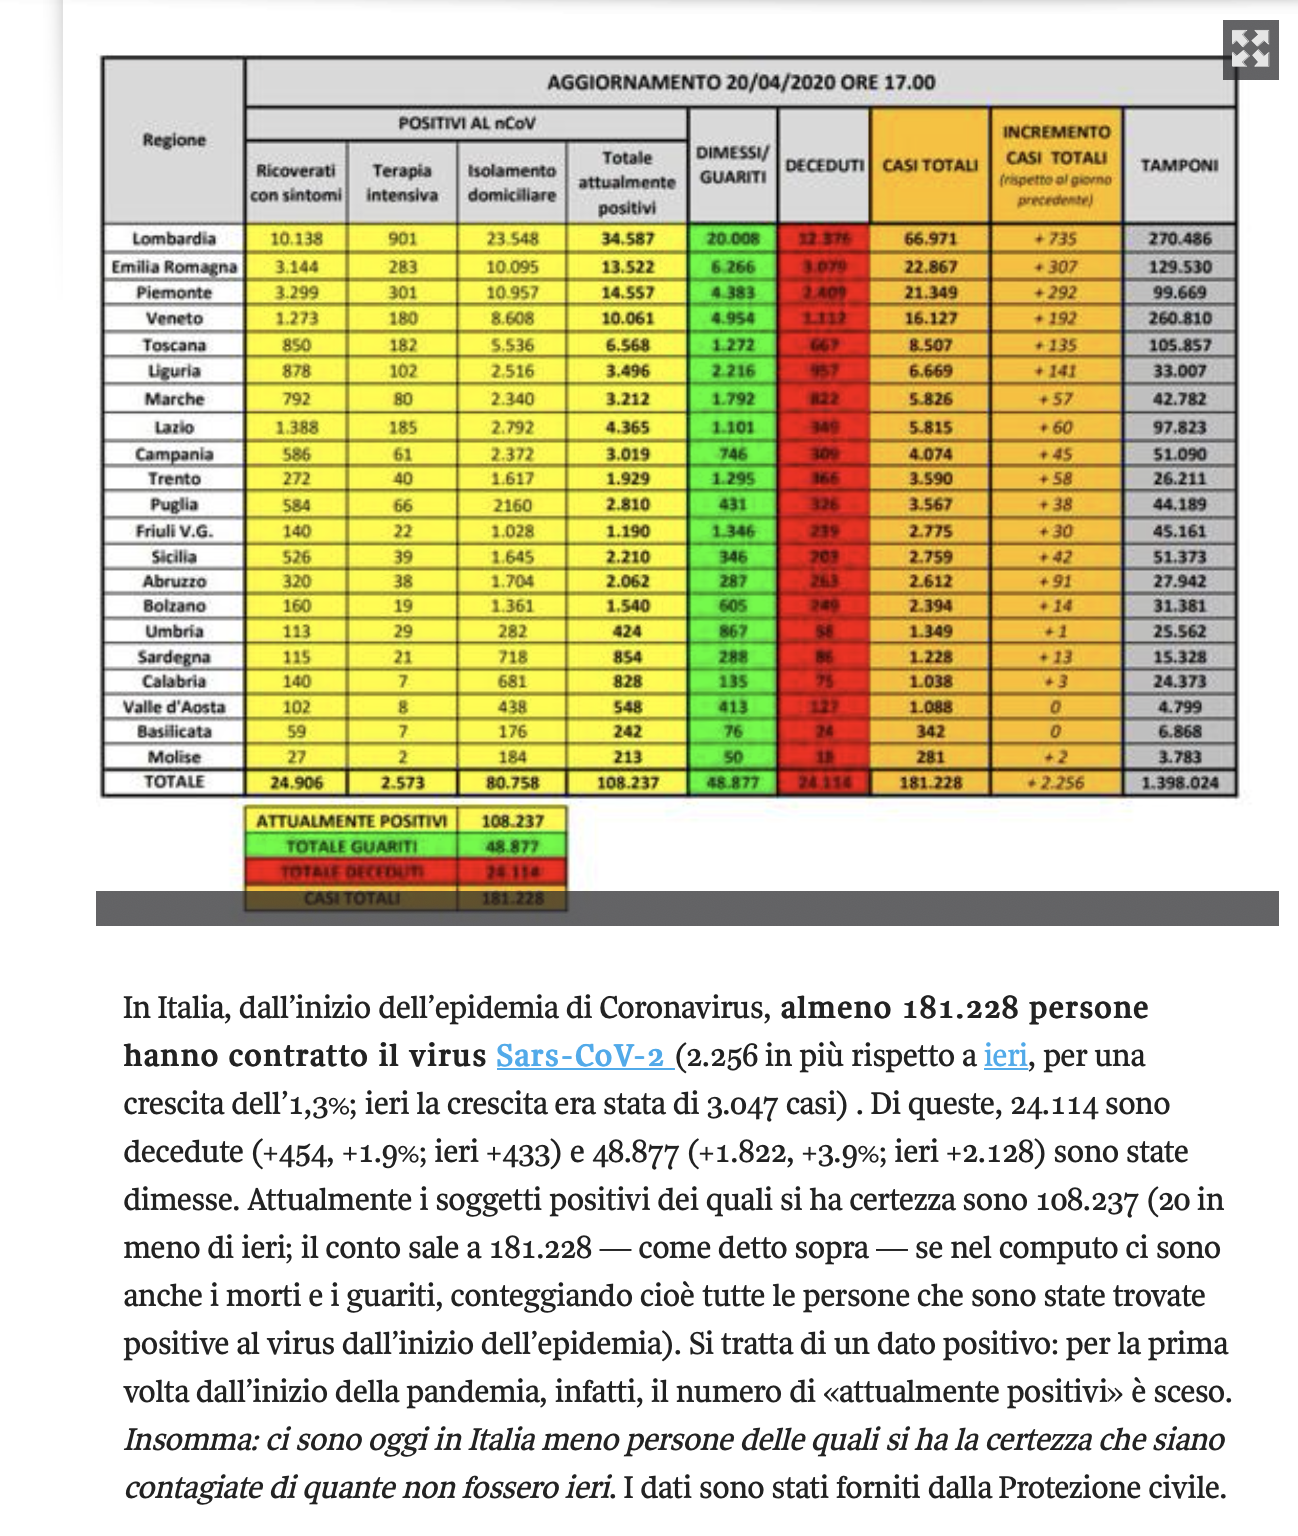
\includegraphics[height=5cm]{img/esempio-articolo-brutto}
				\end{column}
			\end{columns}
		\end{frame}

		\begin{frame}
			\frametitle{Gli strumenti e il modus operandi}
			\framesubtitle{L'importanza e la richiesta di avere ottimi strumenti e il modo di lavorare}
			Abbiamo intervistato diversi giornalisti, sia telefonicamente che tramite un Google Form, per conoscere i loro metodi di lavoro e le loro esigenze.
		\end{frame}

		\begin{frame}
			\frametitle{Task frequenti e significativi}
			\begin{itemize}[<+->]
				\item Comprendere l'andamento della curva epidemiologica\\
				\item Monitorare l'occupazione delle strutture sanitarie\\
				\item Monitorare l'andamento del tasso di letalità\\
				\item Analizzare la distribuzione delle metriche epidemiologiche sulla popolazione\\
				\item Confrontare l'andamento della pandemia tra diverse regioni\\
				\item Confrontare l'andamento della pandemia tra diversi periodi temporali\\
			\end{itemize}
		\end{frame}


	\section{Analisi risorse esistenti}
		\subsection{Linee guida}

			\begin{frame}
	 			\frametitle{Linee guida}
				Abbiamo individuato un totale di \textbf{42} linee guida che si adattano alla progettazione di una dashboard.
				\begin{block}{Fonti delle linee guida}
					\begin{itemize}[<+->]
						\item A. Dix et alii, HCI, Prentice Hall, 1998\\
						\item Jeff Johnson, Designing with the mind in mind, Morgan Kaufmann, 2010\\
						\item D. Egan, “Individual differences in HCI”, in M. Helander (ed.), Handbook of HCI, North-Holland, 1988\\
						\item A. Vaisman, E. Zimanyi. Data Warehouse System: Design and Implementation. Springer, 2016\\
						\item The guidelines of UserFocus.co.uk (commercial, UK, 2014)\\
						\item The 10 heuristics of Nielsen and Molich (1994)\\
						\item The 20 heuristics of Weinshenk and Barker (2000)\\
					\end{itemize}
				\end{block}
			\end{frame}
		
			\begin{frame}
				\frametitle{Valutazione delle risorse esistenti}
				Abbiamo analizzato l'interfaccia di una delle dashboard maggiormente utilizzate dai giornalisti, ossia la Dashboard "Situazione Italia'' curata dal Dipartimento della Protezione Civile (DPC). \newline \newline
				Abbiamo individuato la violazione di ben 23 linee guida sulle 42 valutate e svariate altre criticità. 
			\end{frame}

			\begin{frame}
				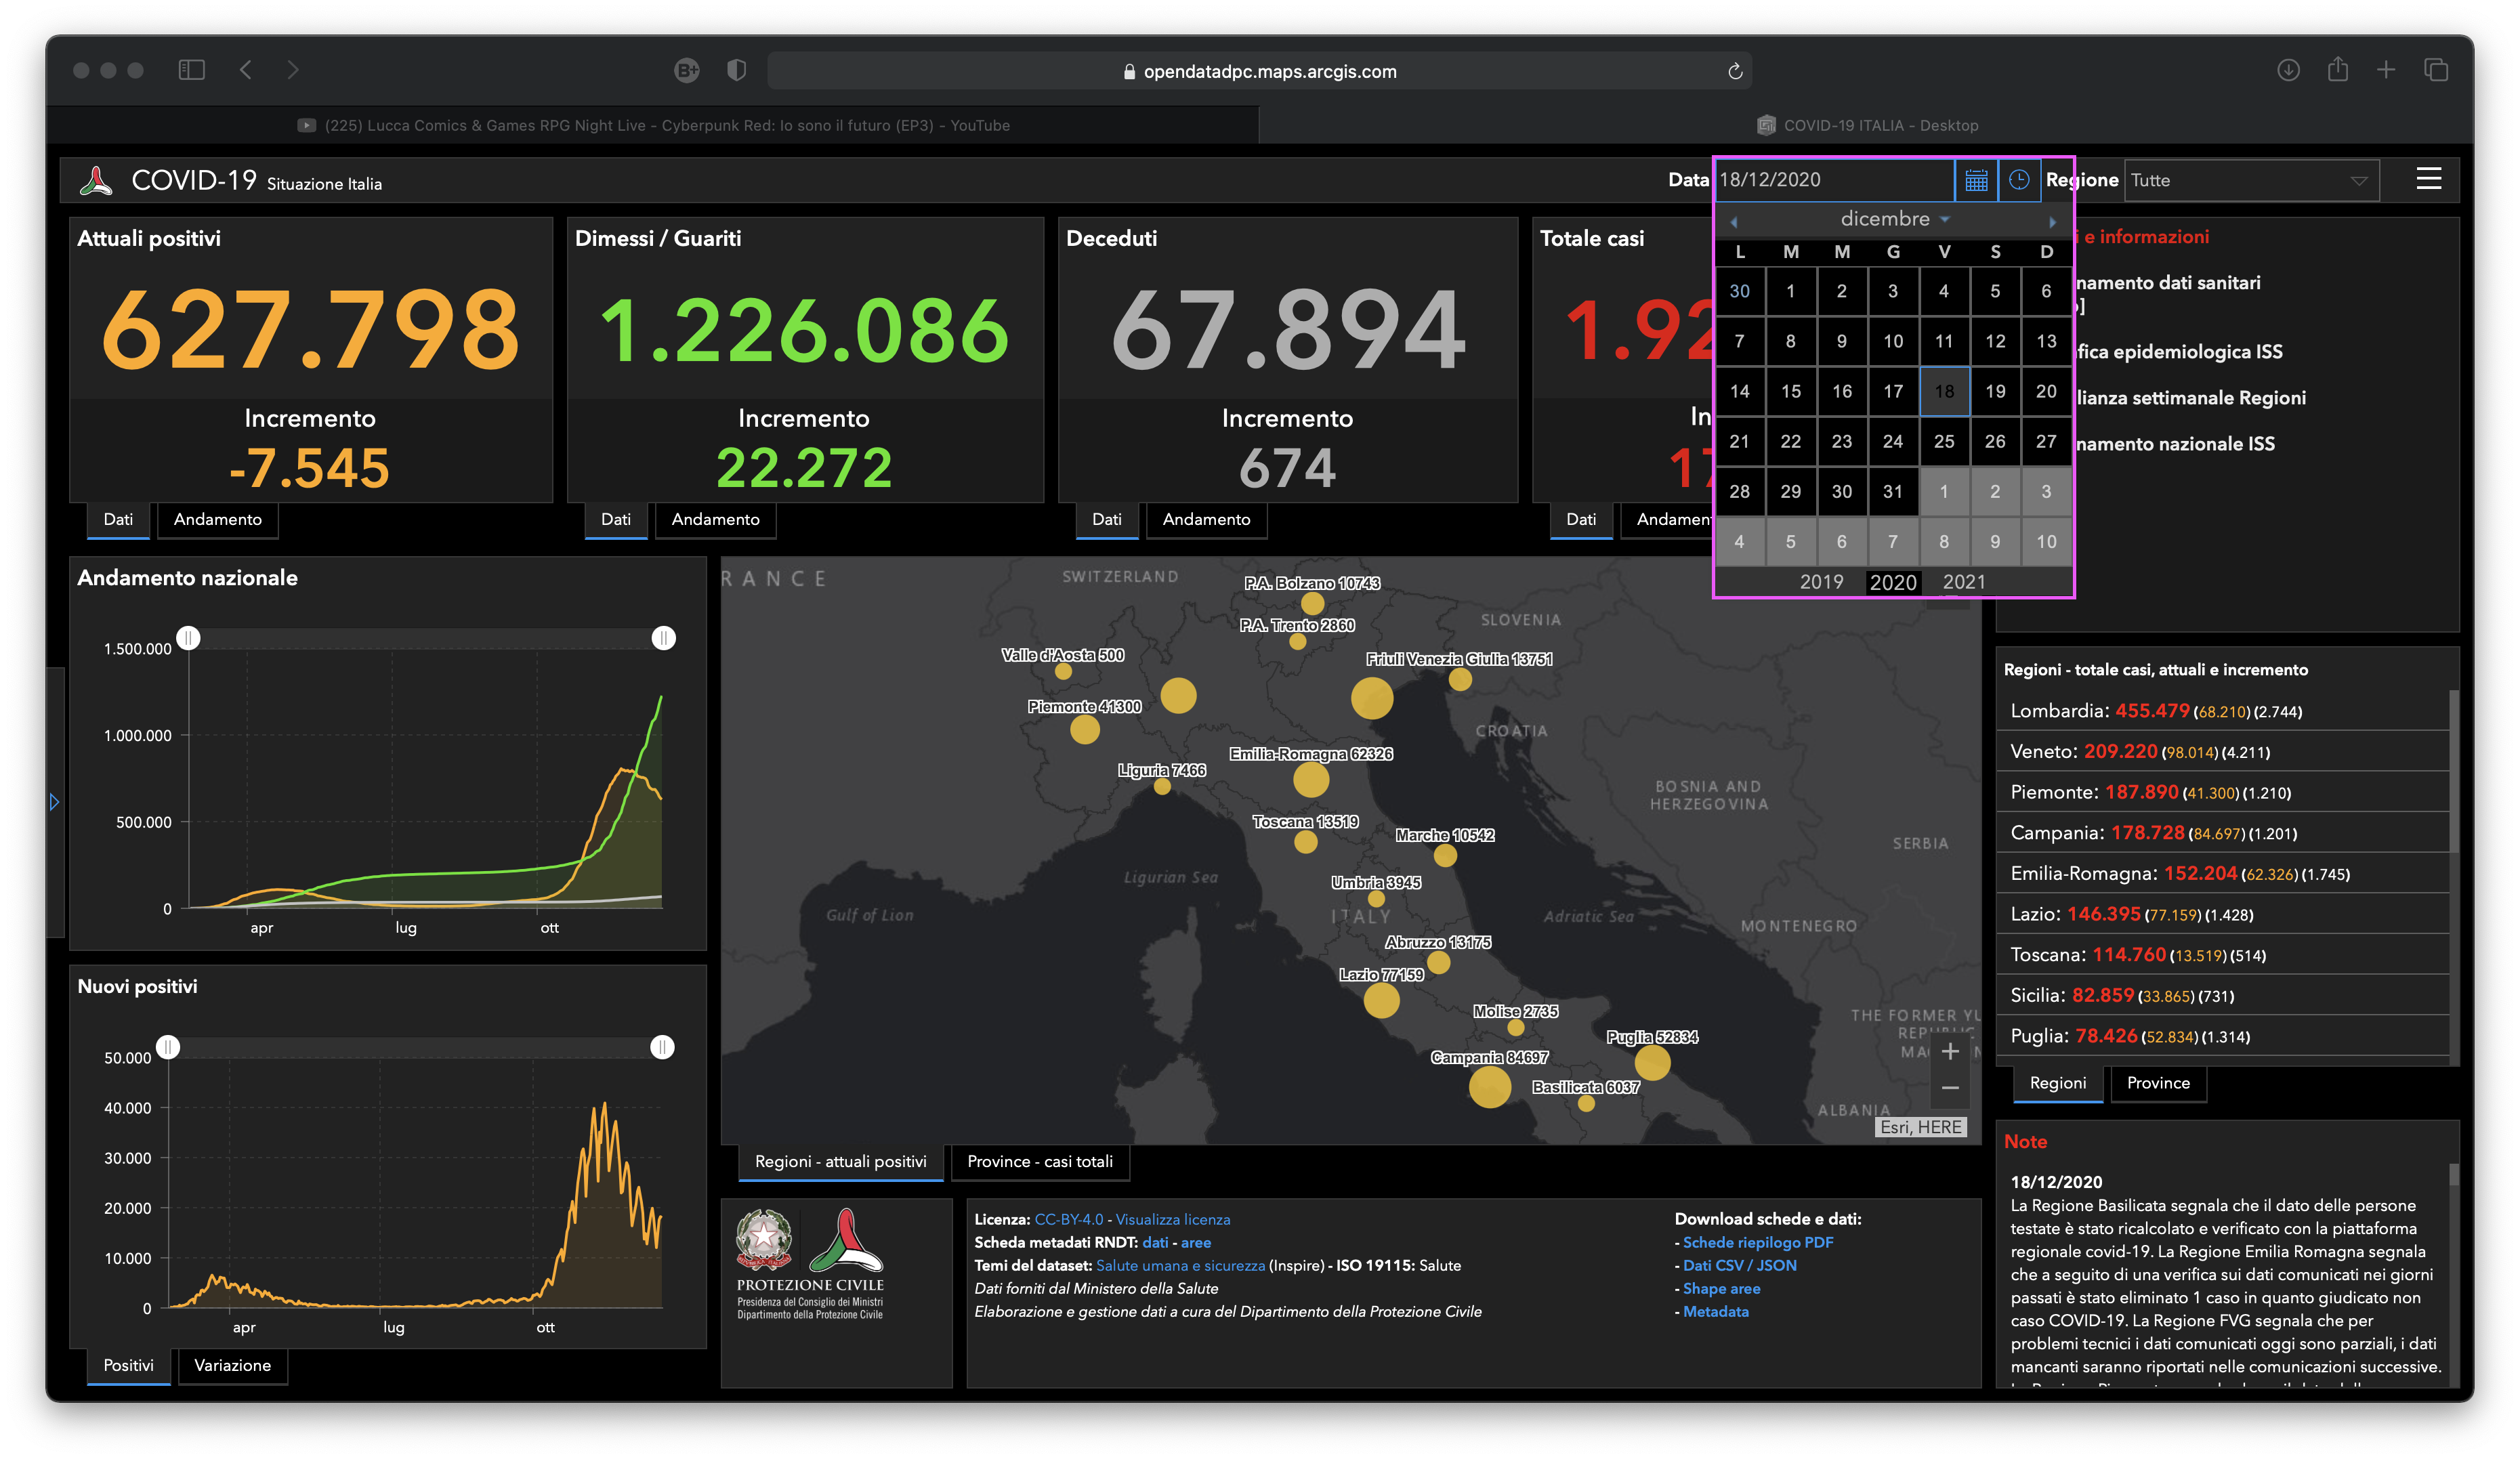
\includegraphics[width=10cm]{img/guidelines_violations_8}	
			\end{frame}

			\begin{frame}
				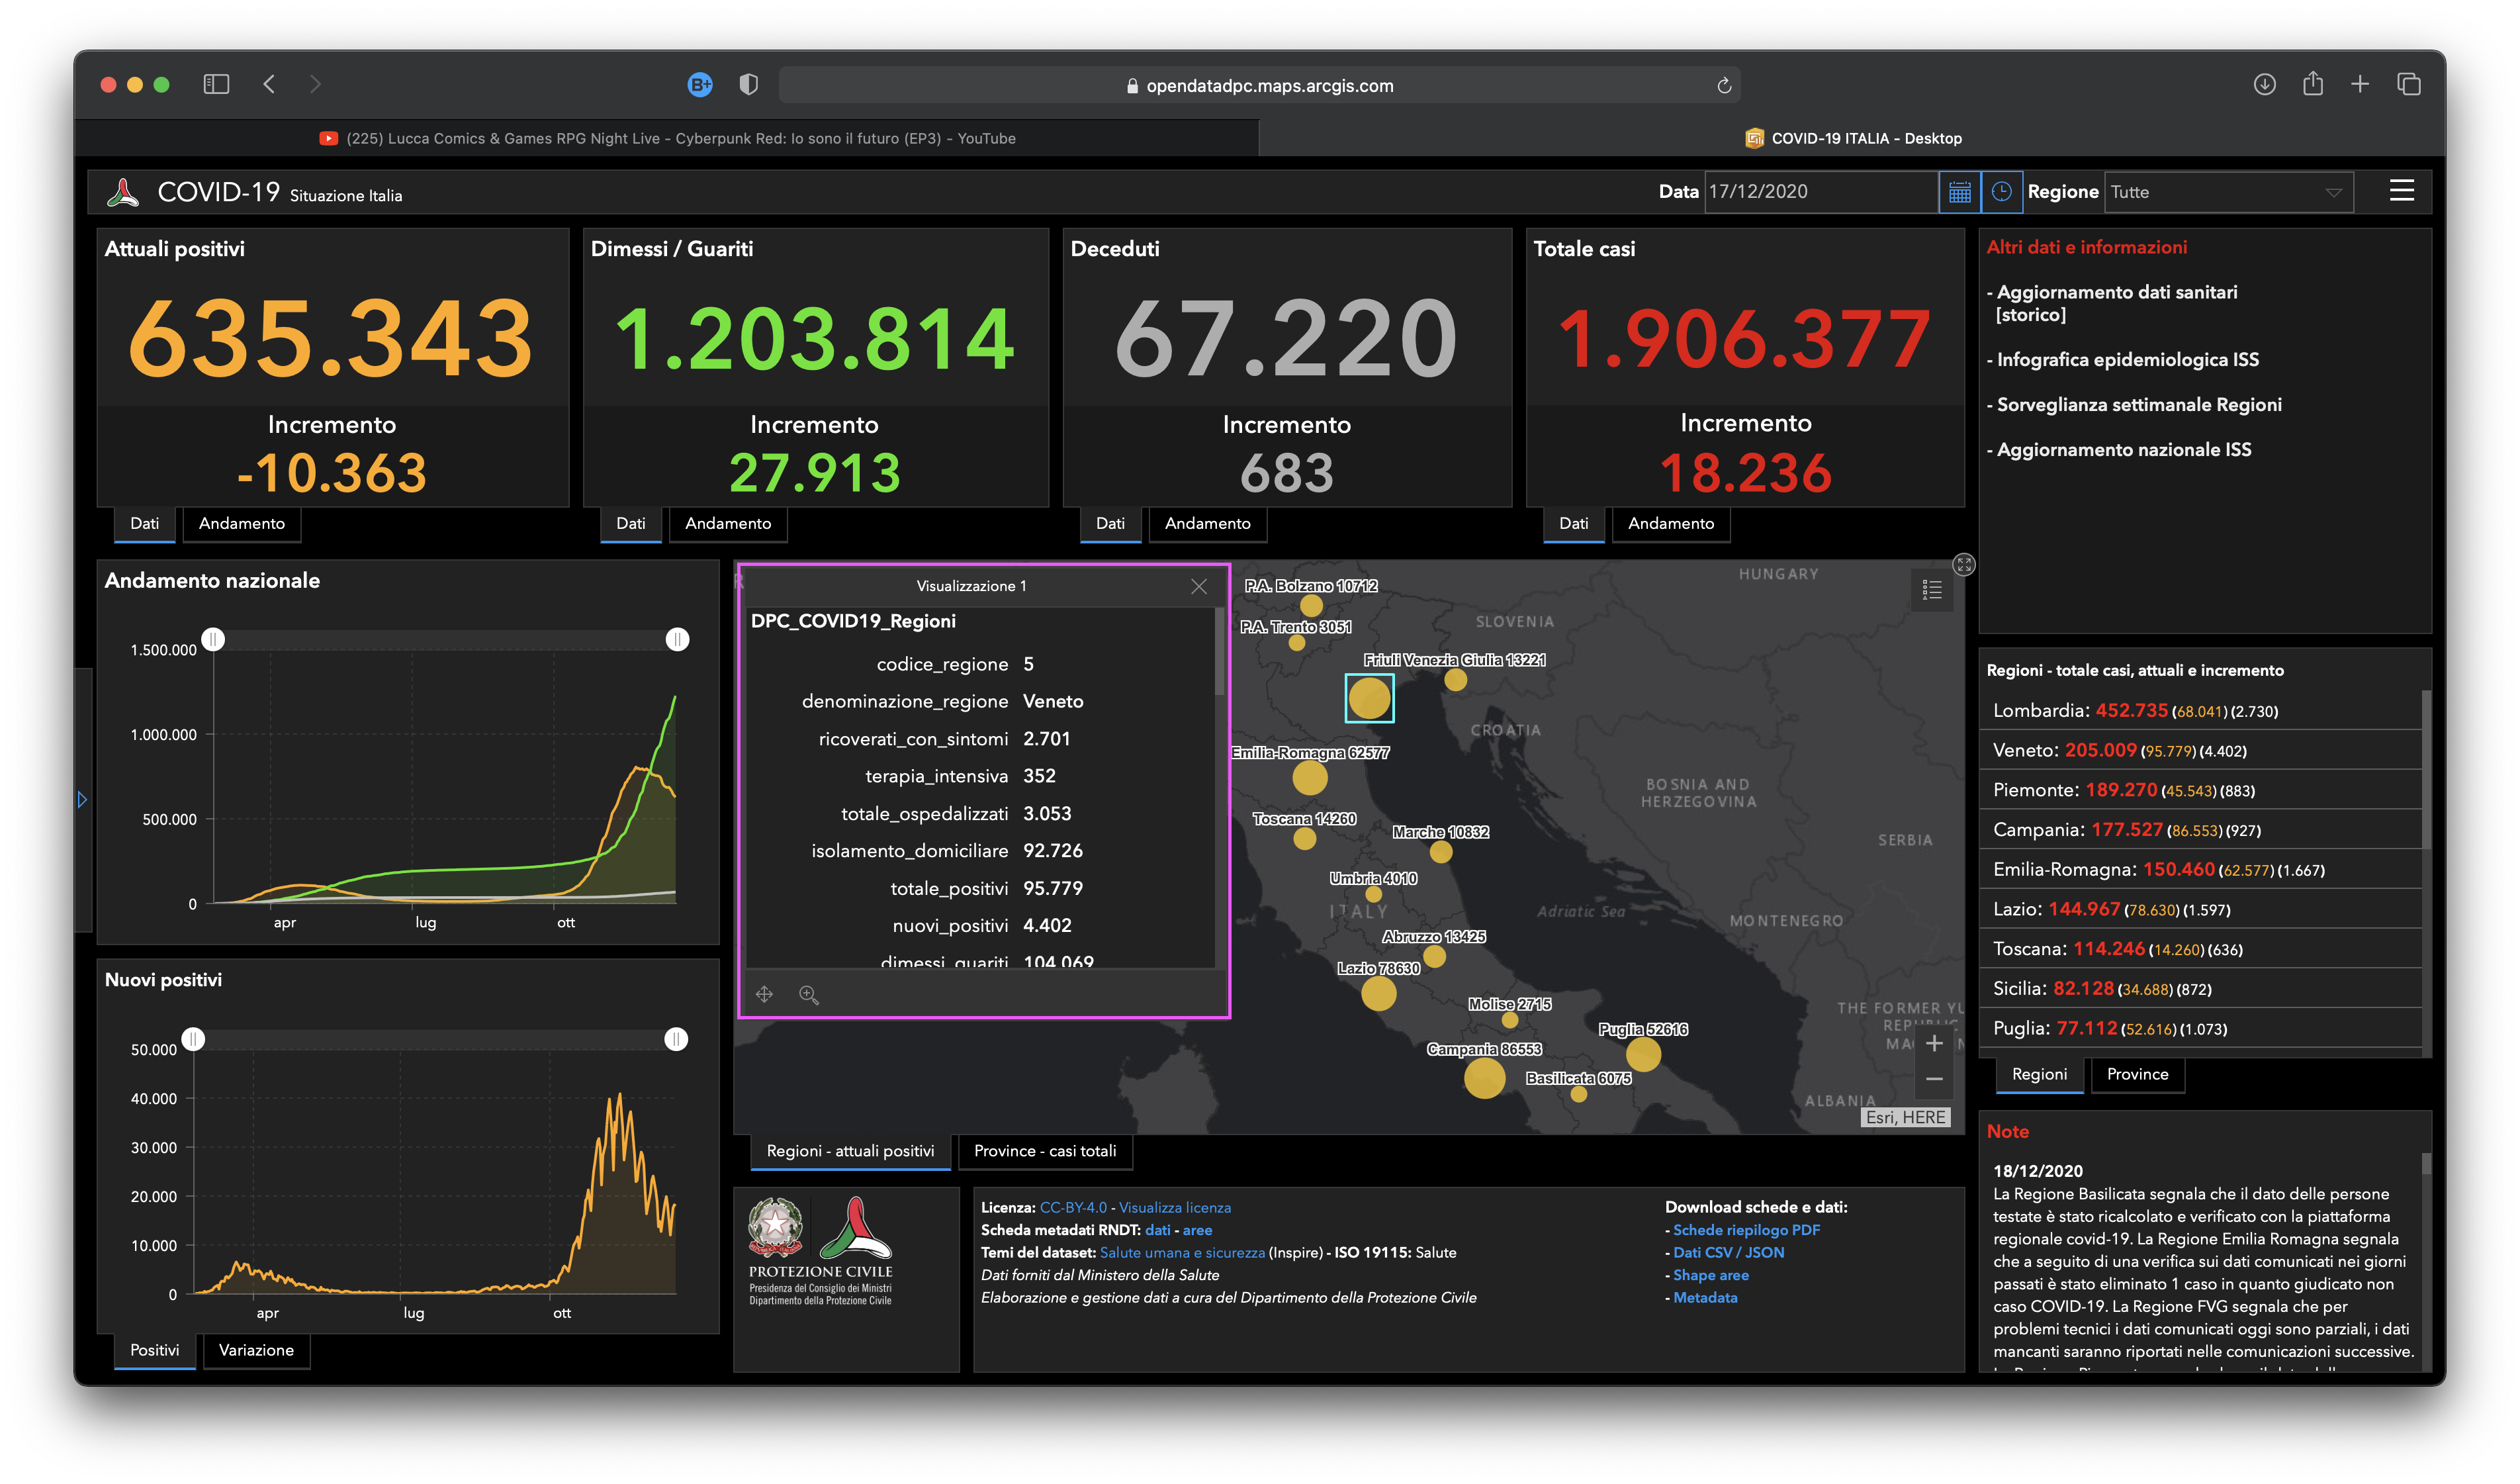
\includegraphics[width=10cm]{img/guidelines_violations_10}
			\end{frame}


		\subsection{Testing con gli utenti}

			\begin{frame}
				\frametitle{Testing con gli utenti}
				Abbiamo chiesto ad alcuni giornalisti di svolgere i task sulla dashboard attuale al fine di raccogliere evidenze circa le criticità da risolvere e gli aspetti da migliorare. \newline \newline
				Abbiamo adottato l'approccio \textit{Guerrilla Usability Testing} per registrare gli errori compiuti dai tester e, quindi, definire una \textbf{curva delle urgenze}.
			\end{frame}

			\begin{frame}
				\frametitle{Curva delle urgenze}
				\begin{columns}[t]
					\begin{column}[T]{5cm}
						Abbiamo valutato i dati raccolti calcolando la frequenza degli errori e assegnando loro una misura dell'impatto sul completamento dei task, per poi riportali su un piano cartesiano e quindi tracciare la curva di urgenza.
					\end{column}
					\begin{column}[T]{5cm}
						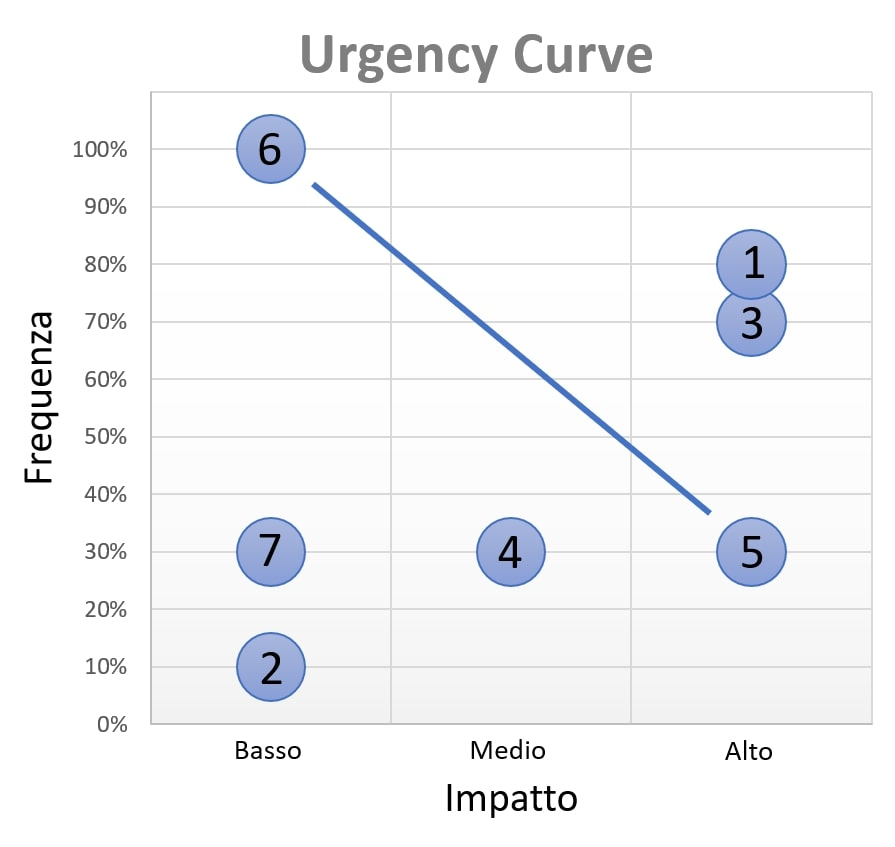
\includegraphics[height=5cm]{img/urgency_curve}
					\end{column}
				\end{columns}
			\end{frame}
		 
			\begin{frame}
				\frametitle{Roadmap}
				\begin{itemize}[<+->]
					\item \textbf{1}: Impossibile trovare il dato ``Tamponi effettuati''\\
					\item \textbf{3}: Impossibile trovare il dato relativo alle disponibilità nelle strutture ospedaliere\\
					\item \textbf{6}: Presenza di etichette poco chiare\\
					\item \textbf{5}: Non tutti i dati sono disponibili nella dashboard
					\item \textbf{4}: \`E lasciato all'utente il compito di computare il tasso di letalità\\
					\item \textbf{7}: \`E lasciato all'utente il compito di computare gli incrementi in un periodo di tempo\\
					\item \textbf{2}: Alcuni dati sono presenti nel PDF raggiungibile ``Schede riepilogo PDF''\\
				\end{itemize}
			\end{frame}

	\section{Studio di fattiblità}
		\subsection{Scenari}
		\begin{frame}
			\frametitle{Scenari}
			\begin{itemize}[<+->]
				\item Analisi dei dati quotidiani sull'andamento dell'epidemia Covid-19 in Italia\\
				\item Analisi dei dati quotidiani sull'andamento dell'epidemia Covid-19 nella regione Emilia Romagna\\
				\item Analisi sull'andamento del tasso di letalità e dei numeri dell'epidemia nelle due settimane precedenti\\
				\item Analisi delle differenze dell'andamento nelle regioni Emilia Romagna, Veneto e Molise nelle precedenti due settimane\\
				\item Analisi delle differenze dell'andamento dell'epidemia in Italia nel mese corrente rispetto ai due precedenti\\
			\end{itemize}
		\end{frame}

		\subsection{Personas}
		\begin{frame}
			\frametitle{Personas}
			Abbiamo individuato un totale di \textbf{6} persona ognuna rappresentante un profilo interessante e peculiare. Trattasi di:
			\begin{itemize}[<+->]
				\item Giornalista di una testata nazionale\\
				\item Giornalista di una testata locale\\
				\item Giornalista d'agenzia\\
				\item Blogger (persona secondaria)\\
				\item Cittadino esperto (persona addizionale)\\
				\item Utente che accede alla dashboard da un dispositivo mobile (persona addizionale)\\
			\end{itemize}
		\end{frame}

		\begin{frame}
			\frametitle{Giovanni}
			\begin{columns}[t]
				\begin{column}[T]{6cm}
					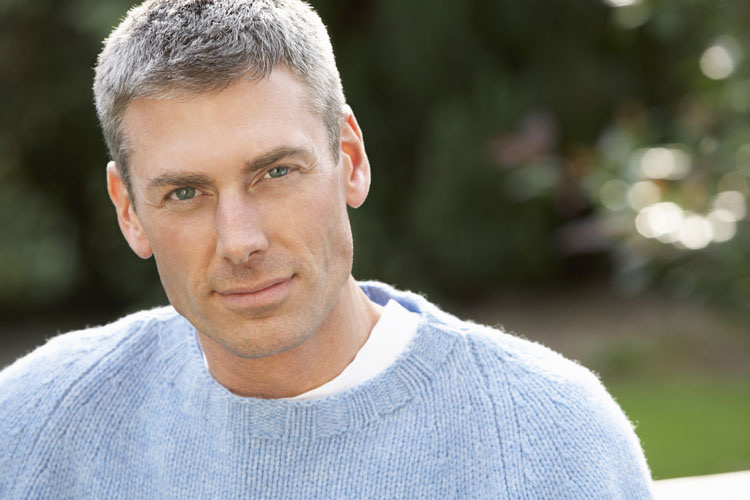
\includegraphics[height=2.5cm]{img/giovanni}
					\textit{``Forza, un altro giorno in cui dovrò dare il massimo per scrivere un ottimo articolo.''}\\
					Giovanni è un utente ormai esperto di dashboard, ne visita diverse e sceglie solo quella che gli permette di comprendere più velocemente e profondamente il quadro epidemiologico.
				\end{column}
				\begin{column}[T]{5cm}
					\textbf{Età:} 53\\
					\textbf{Occupazione:} Articolista presso una testata nazionale\\
					\textbf{Famiglia:} Sposato e con due figlie\\
					\textbf{Profilo tecnico:} Esperto ed esigente, in ufficio usa un computer fisso con uno schermo da 24 pollici\\
				\end{column}
			\end{columns}
		\end{frame}

		\begin{frame}
			\frametitle{Francesca}
			\begin{columns}[t]
				\begin{column}[T]{6cm}
					
\includegraphics[height=2.5cm]{img/francesca}
					\textit{``Che fatica districarsi tra tutti questi dati, chissà se esiste uno strumento che possa aiutarmi.''}\\
					Francesca è una donna che scrive per il giornale letto nella provincia di Padova, non dà troppo peso ai dati e si informa dove le capita.
				\end{column}
				\begin{column}[T]{5cm}
					\textbf{Età:} 35\\
					\textbf{Occupazione:} Articolista presso una testata locale\\
					\textbf{Famiglia:} Single\\
					\textbf{Profilo tecnico:} Non a suo agio con gli strumenti tecnologici, li usa lo stretto indispensabile\\
				\end{column}
			\end{columns}
		\end{frame}

		\begin{frame}
			\frametitle{Giulia}
			\begin{columns}[t]
				\begin{column}[T]{6cm}
					
\includegraphics[height=3cm]{img/giulia}
					\textit{``Non mi fido di questo dato, si discosta troppo da quello che hanno pubblicato ieri, controlliamo che non ci siano errori.''}\\
					Giulia si occupa di ``fact-checking'' all'interno di un'agenzia di stampa e studia i dati relativi alla pandemia Covid-19.
				\end{column}
				\begin{column}[T]{5cm}
					\textbf{Età:} 35\\
					\textbf{Occupazione:} Articolista e ``fact-checker'' presso un'agenzia di stampa\\
					\textbf{Famiglia:} Convivente\\
					\textbf{Profilo tecnico:} Esperta e familiare con le ultime tecnologie, spronata a tenersi al passo anche dal suo ambiente di lavoro\\
				\end{column}
			\end{columns}
		\end{frame}

		\begin{frame}
			\frametitle{Roberto}
			\begin{columns}[t]
				\begin{column}[T]{6cm}
					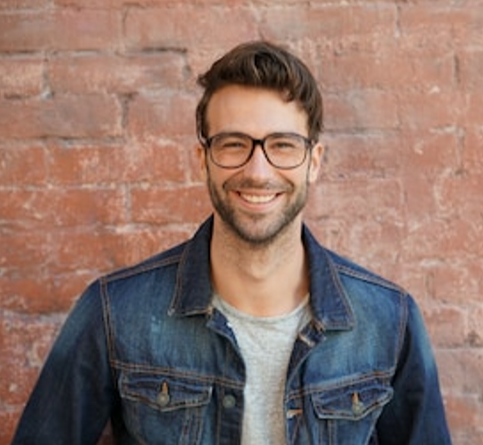
\includegraphics[height=3cm]{img/francesco}
					\textit{``I miei follower mi hanno chiesto un video sul Covid, vediamo un po' qual è l'andamento in Italia.''}\\
					Roberto è un giovane utente con un blog e un canale YouTube in cui tratta argomenti di attualità.
				\end{column}
				\begin{column}[T]{5cm}
					\textbf{Età:} 30\\
					\textbf{Occupazione:} Blogger e YouTuber\\
					\textbf{Famiglia:} Convivente\\
					\textbf{Profilo tecnico:} Pratico di internet e di strumenti di editing\\
				\end{column}
			\end{columns}
		\end{frame}

		\begin{frame}
			\frametitle{Fabio}
			\begin{columns}[t]
				\begin{column}[T]{6cm}
					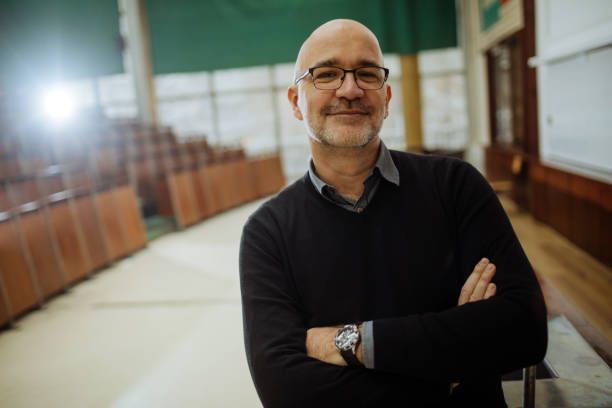
\includegraphics[height=2.5cm]{img/fabio}
					\textit{``Questi dati sono molto interessanti, vorrei condividerli sul mio profilo Twitter per farli vedere a tutti.''}\\
					Fabio è una persona alla quale piace tenersi aggiornato sugli ultimi fatti che accadono nel mondo e nella sua città.
				\end{column}
				\begin{column}[T]{5cm}
					\textbf{Età:} 62\\
					\textbf{Occupazione:} Professore universitario di informatica\\
					\textbf{Famiglia:} Sposato e con due figli\\
					\textbf{Profilo tecnico:} Esperto ma non più agile nell'apprendere il funzionamento di nuovi strumenti\\
				\end{column}
			\end{columns}
		\end{frame}

		\begin{frame}
			\frametitle{Christian}
			\begin{columns}[t]
				\begin{column}[T]{6cm}
					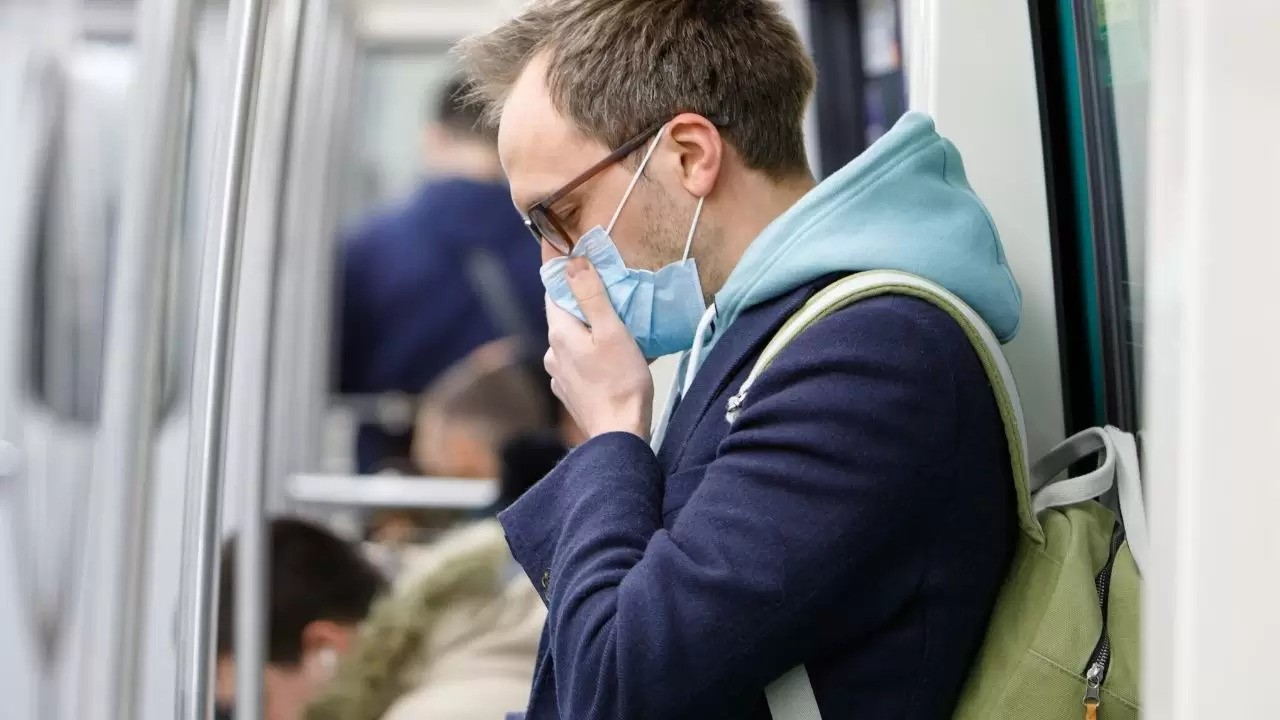
\includegraphics[height=2.5cm]{img/christian}
					\textit{``Che giornata stancante, chissà cos'è successo oggi nel mondo, aprirò il mio feed Facebook per vedere le ultime novità''}\\
					Christian è un assiduo utilizzatore di smartphone e  ha tempo solo alla sera per aggiornarsi su quanto accade attorno a lui.
				\end{column}
				\begin{column}[T]{5cm}
					\textbf{Età:} 34\\
					\textbf{Occupazione:} Corriere\\
					\textbf{Famiglia:} Single\\
					\textbf{Profilo tecnico:} Poco familiare con la tecnologia, utilizza esclusivamente lo smartphone\\
				\end{column}
			\end{columns}
		\end{frame}
		
	\section{Progettazione proposta}
		%\subsection{Design model}
		\begin{frame}
			\frametitle{Design model - CAO=S}
			\begin{enumerate}[<+->]
				\item Abbiamo individuato \textbf{8} concetti a partire dai dati epidemiologici liberamente disponibili e già usati in altre dashboard\\
				\item Utilizzando le persona e gli scenari abbiamo individuato gli attori e, per ognuno di essi, abbiamo realizzato un diagramma C\&A\\
				\item Abbiamo individuato \textbf{7} operazioni che gli attori possono svolgere\\
				\item Abbiamo individuato le strutture definendo quale attore potesse svolgere quale operazione\\
				\item Abbiamo individuato le strutture dati che dovrebbero essere utilizzate per gestire i diversi tipi di dato\\
			\end{enumerate}
		\end{frame}

		%\subsection{Architettura delle informazioni}
		\begin{frame}
			\frametitle{Architettura delle informazioni}
			\begin{itemize}[<+->]
				\item Approccio \textbf{top-down}\\
				\item Caratteristiche individuate:\\
					\begin{itemize}[<+->]
						\item Strutturazione: elementi interattivi\\
						\item Classificazioni: dati aggregati, dati assoluti, dati relativi, serie temporali\\
						\item Organizzazione: utilizzo di componenti grafiche distinte\\
						\item Ricercabilità: non presenti in quanto è mostrato l'intero contenuto informativo\\
						\item Gestione: configurabilità del layout per visioni personalizzate\\
					\end{itemize}
				\item Struttura di tipo \textbf{table of content}\\
			\end{itemize}
		\end{frame}

		%\subsection{Interaction design}
		\begin{frame}
			\frametitle{Interaction design}		
			\begin{itemize}[<+->]
				\item \textbf{Ergonomia}:
				\begin{itemize}[<+->]
					\item Organizzazione controlli e display: raggruppamento per frequenza\\
					\item Condizione ambiente fisico: non impattabile in quanto applicazione web-based\\
					\item Uso dei colori: il colore non è l'unico mezzo per differenziare le componenti\\
				\end{itemize} 
				\item \textbf{Progettazione della conversazione}:
					\begin{enumerate}[<+->]
						\item Menù e navigazione
						\item Manipolazione diretta
					\end{enumerate}
				\item \textbf{Progettazione delle schermate}
				\item \textbf{Contesto sociale e dell'organizzazione}
			\end{itemize}
		\end{frame}

		\subsection{Blueprint}
		\begin{frame}
			\frametitle{Blueprint}
			La realizzazione dei bluprint ha richiesto  tre iterazioni, alla fine delle quali siamo giunti a due blueprint, uno volto all'indicazione dei contenuti di ogni pagina e l'altro rivolto ai programmatori e che esplicita le componenti di ogni pagina.
		\end{frame}

		\begin{frame}
			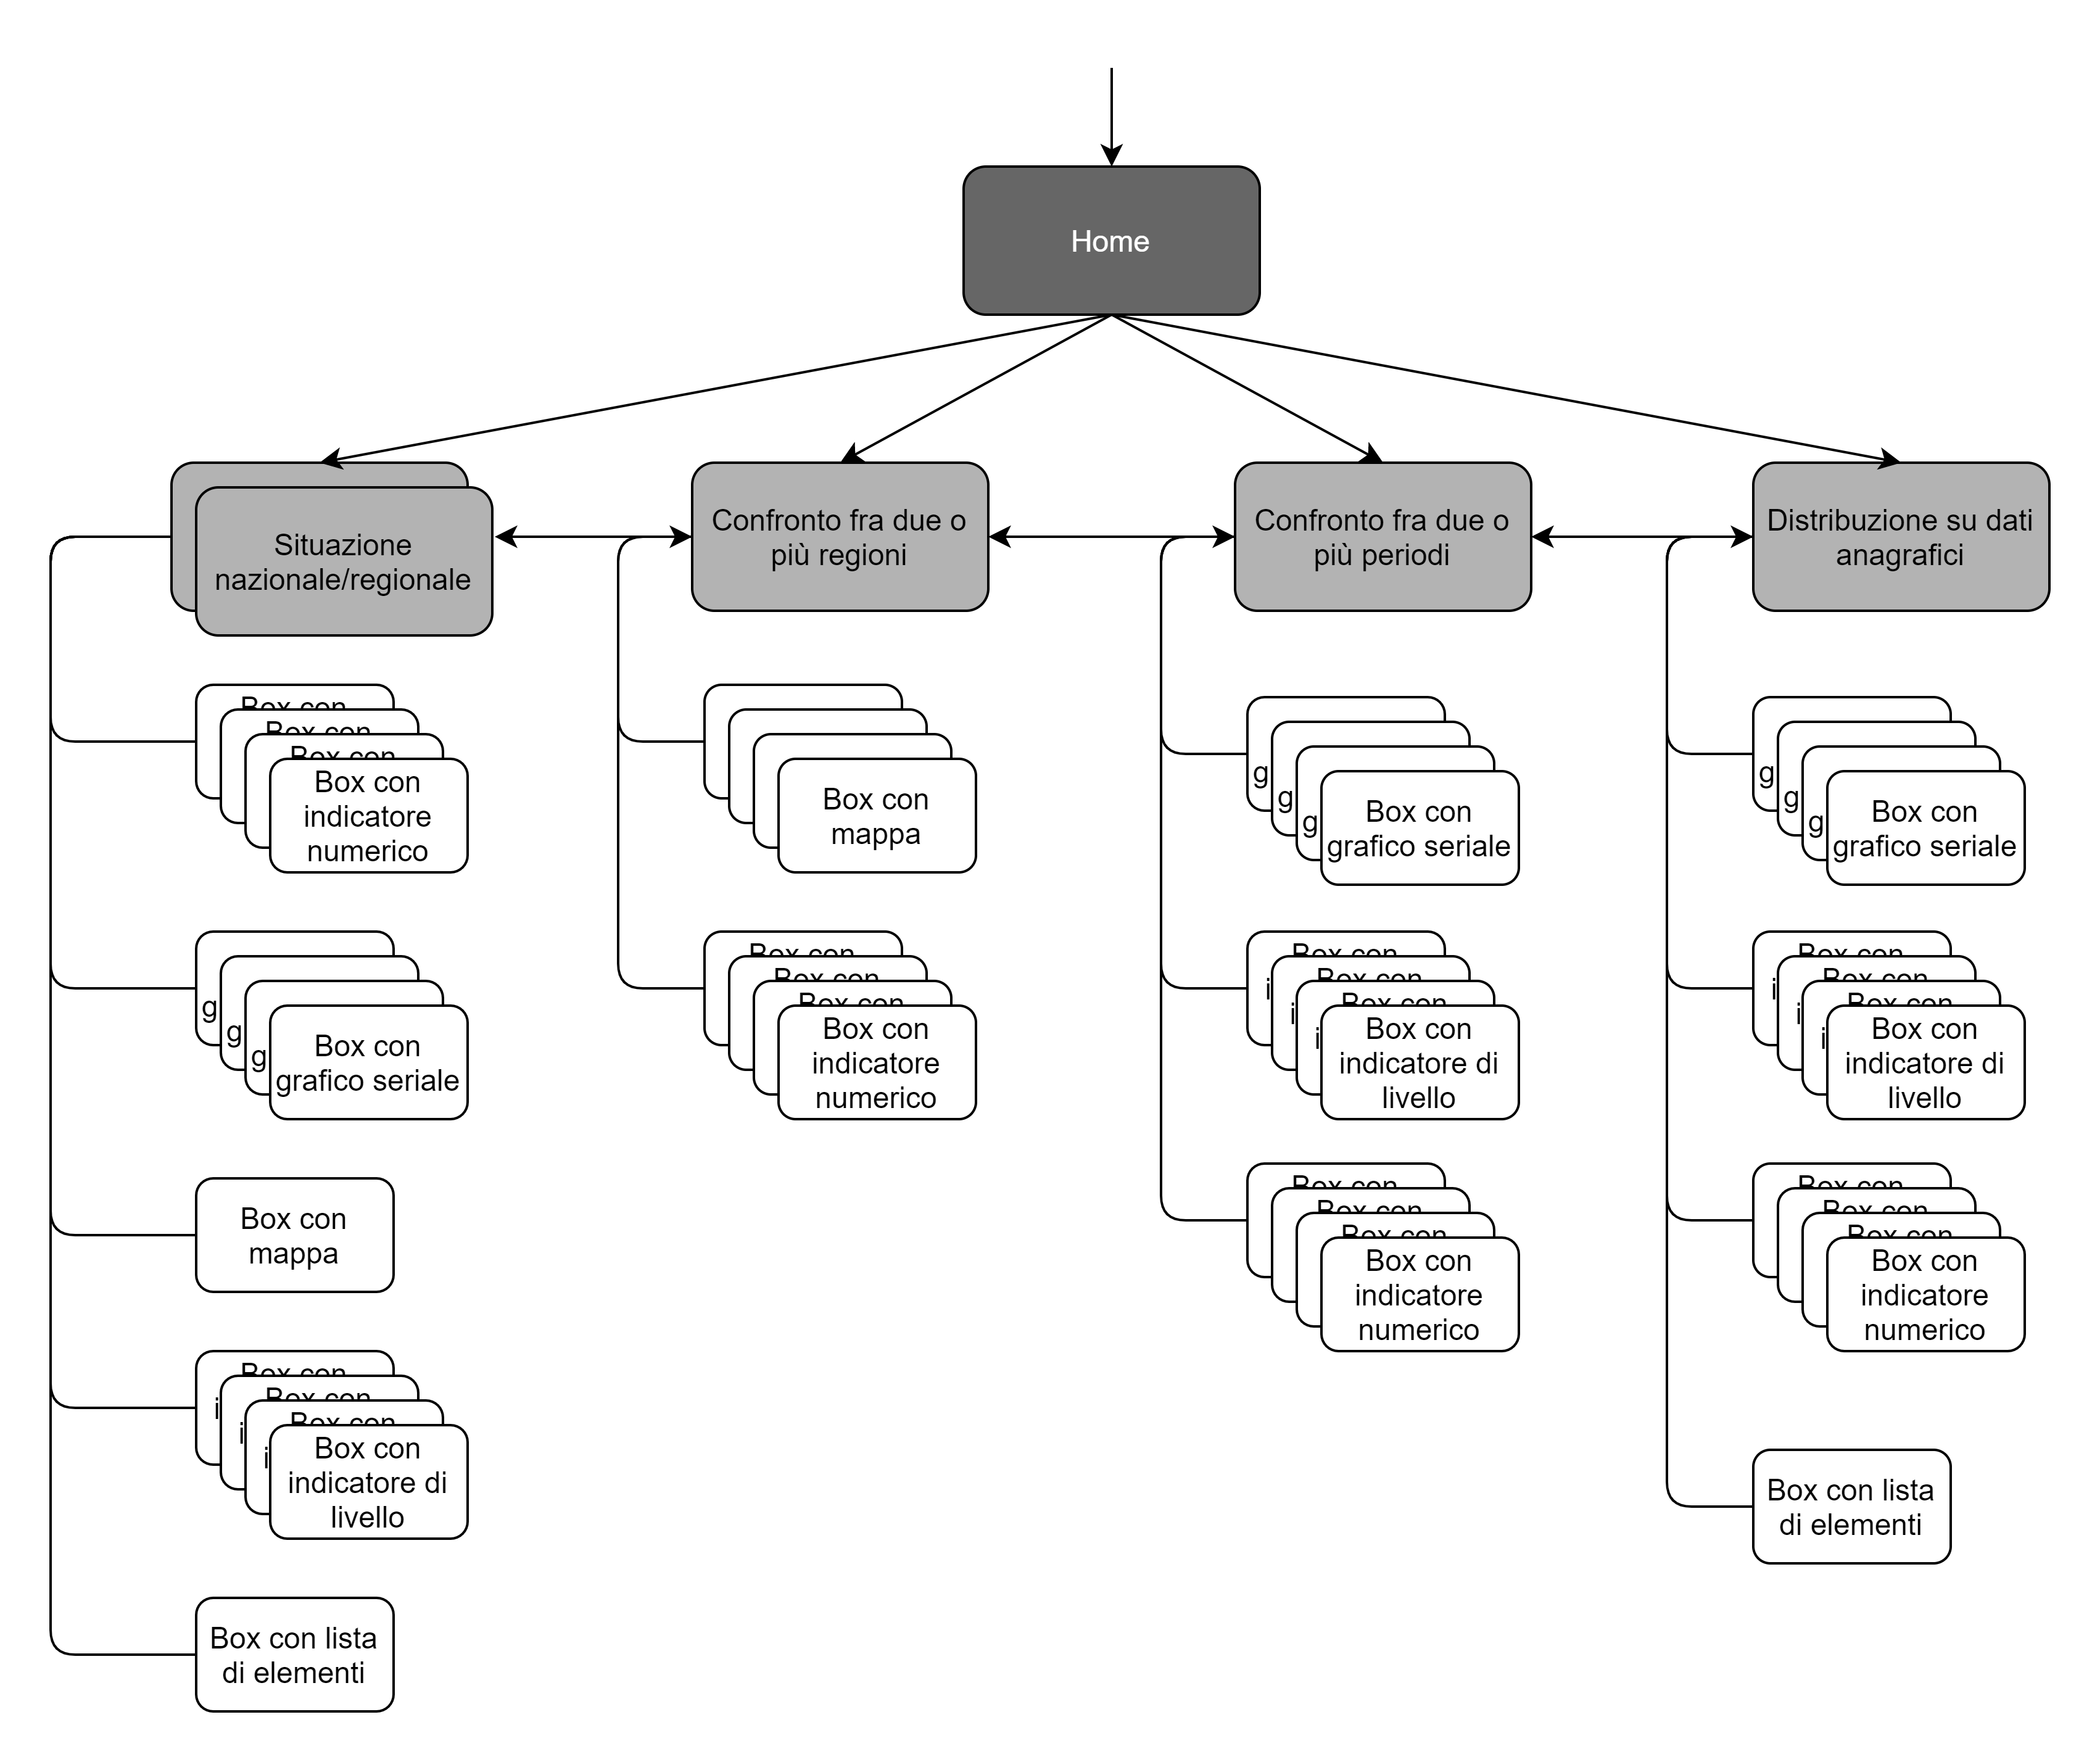
\includegraphics[width=9cm]{img/blueprint-prog-1}
		\end{frame}

		\begin{frame}
			\begin{columns}[t]
					\begin{column}[T]{5cm}
						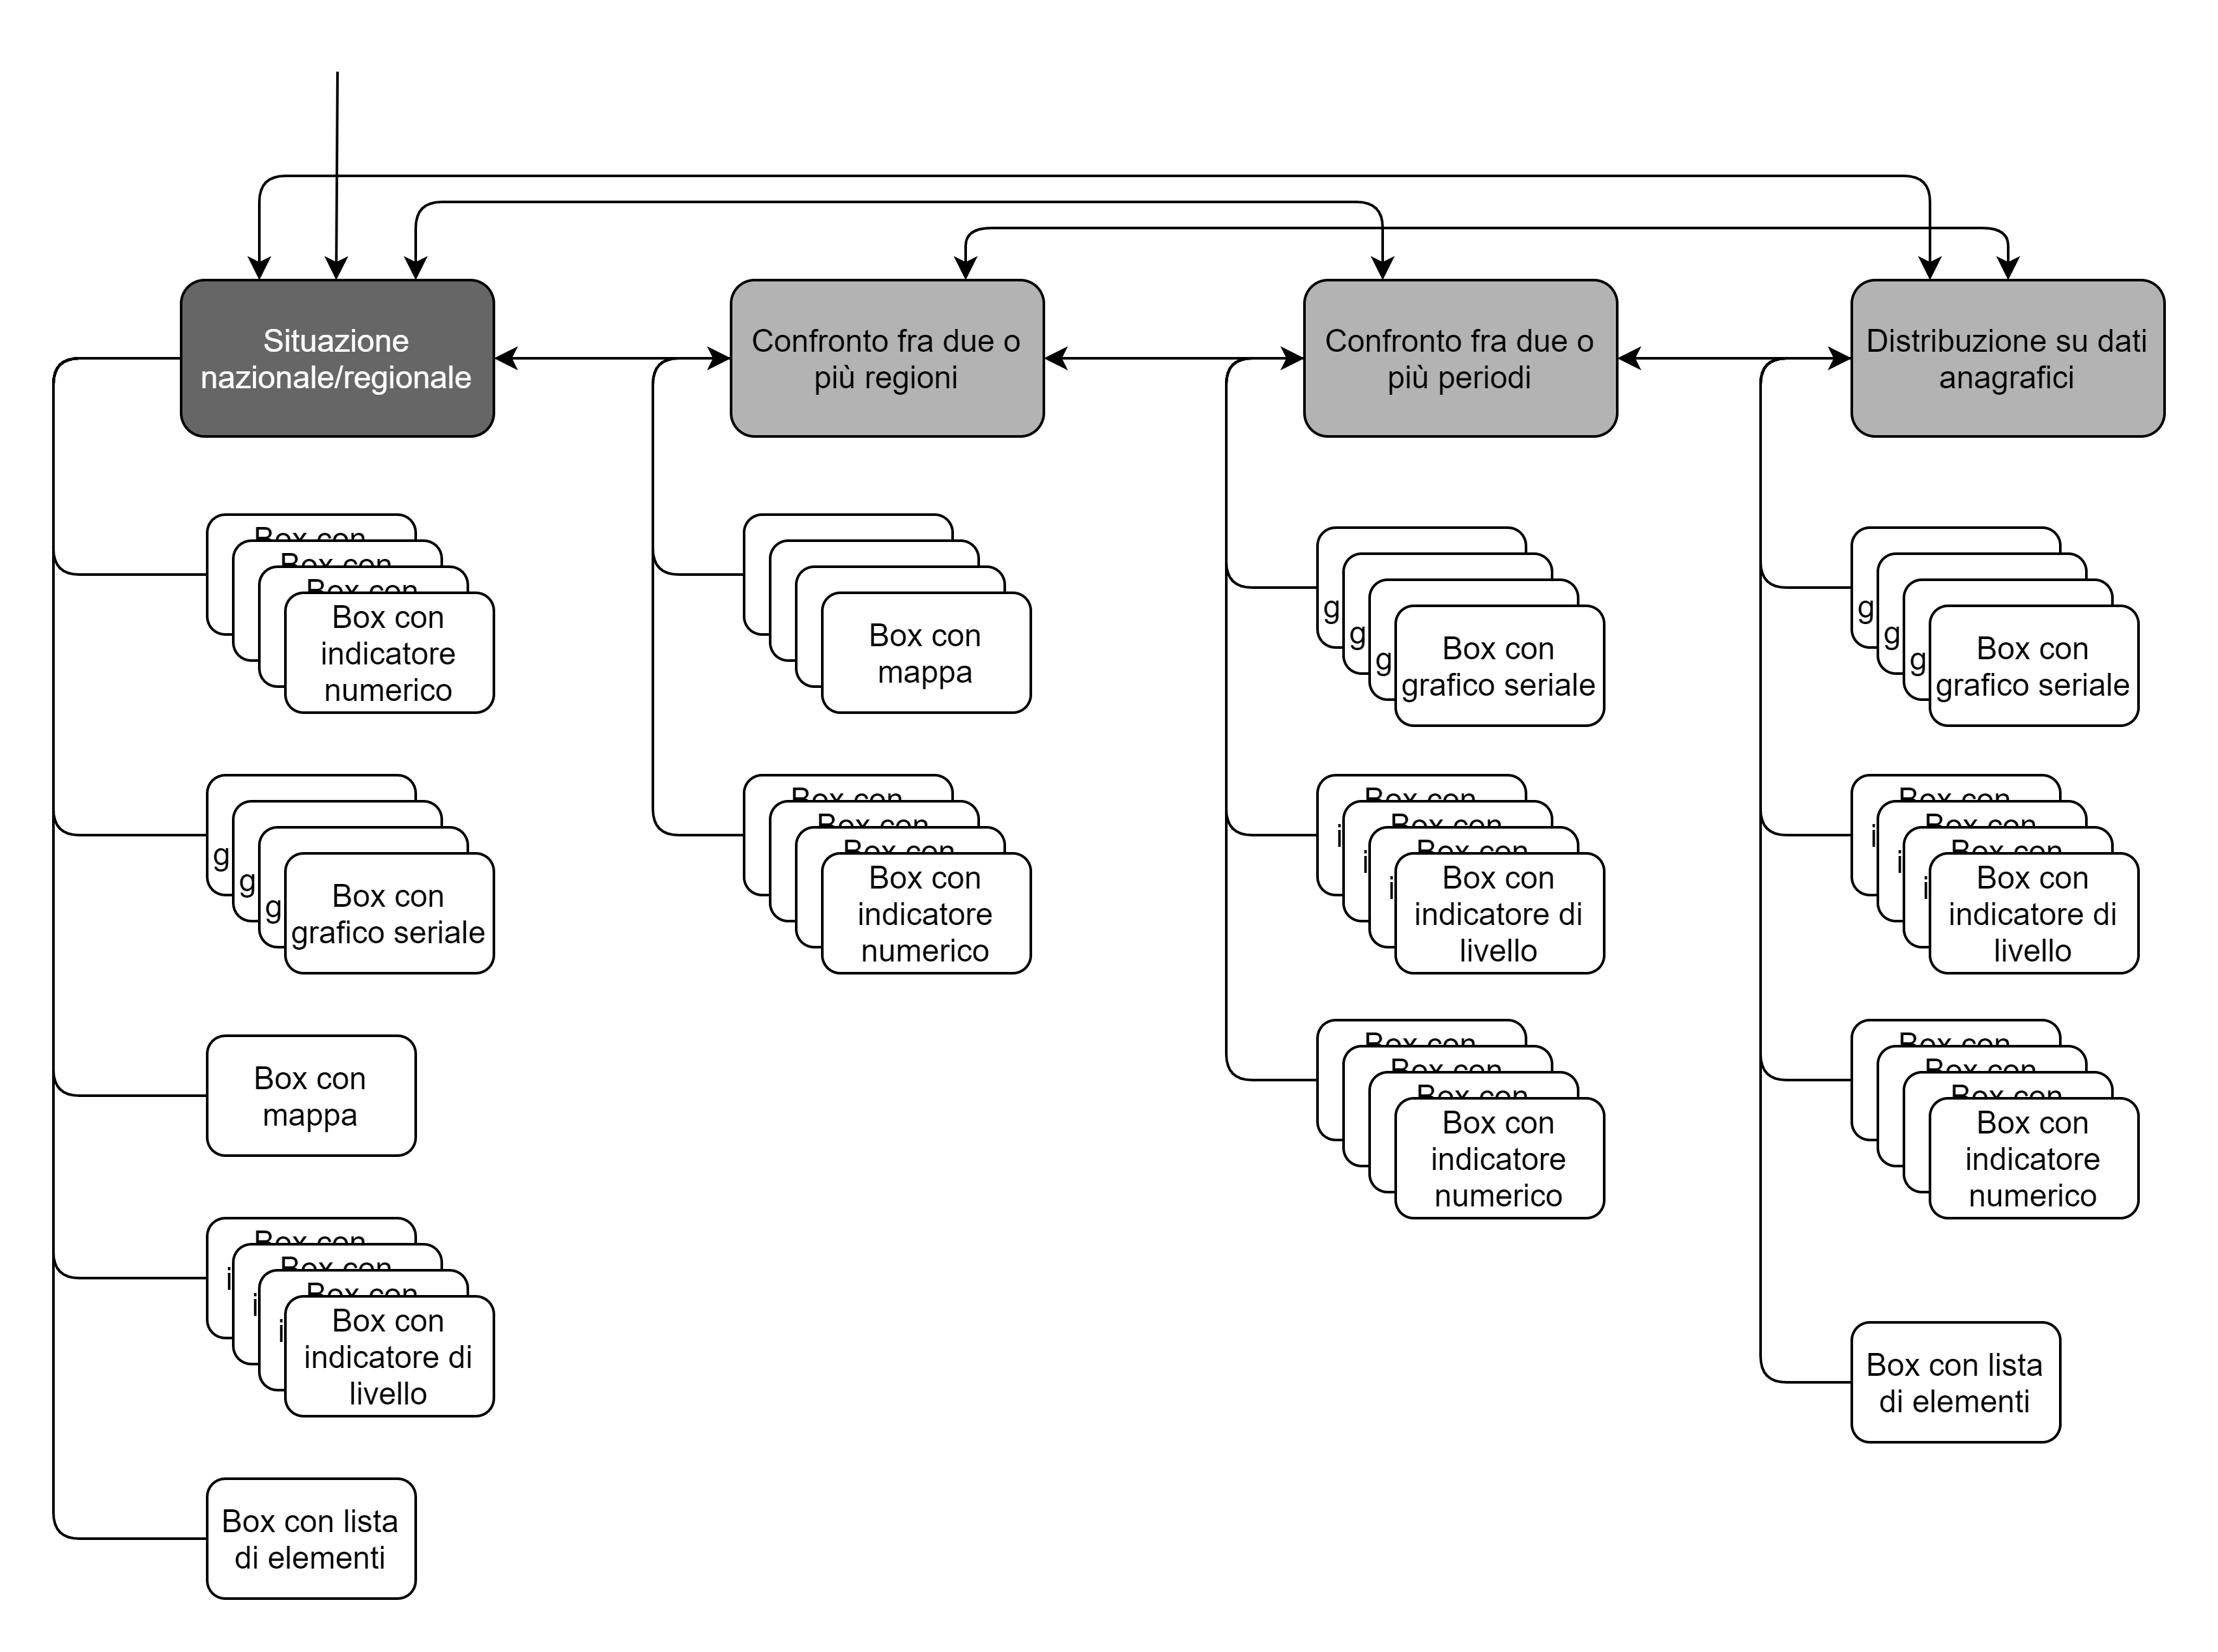
\includegraphics[width=5cm]{img/blueprint-prog-2}
					\end{column}
					\begin{column}[T]{5cm}
						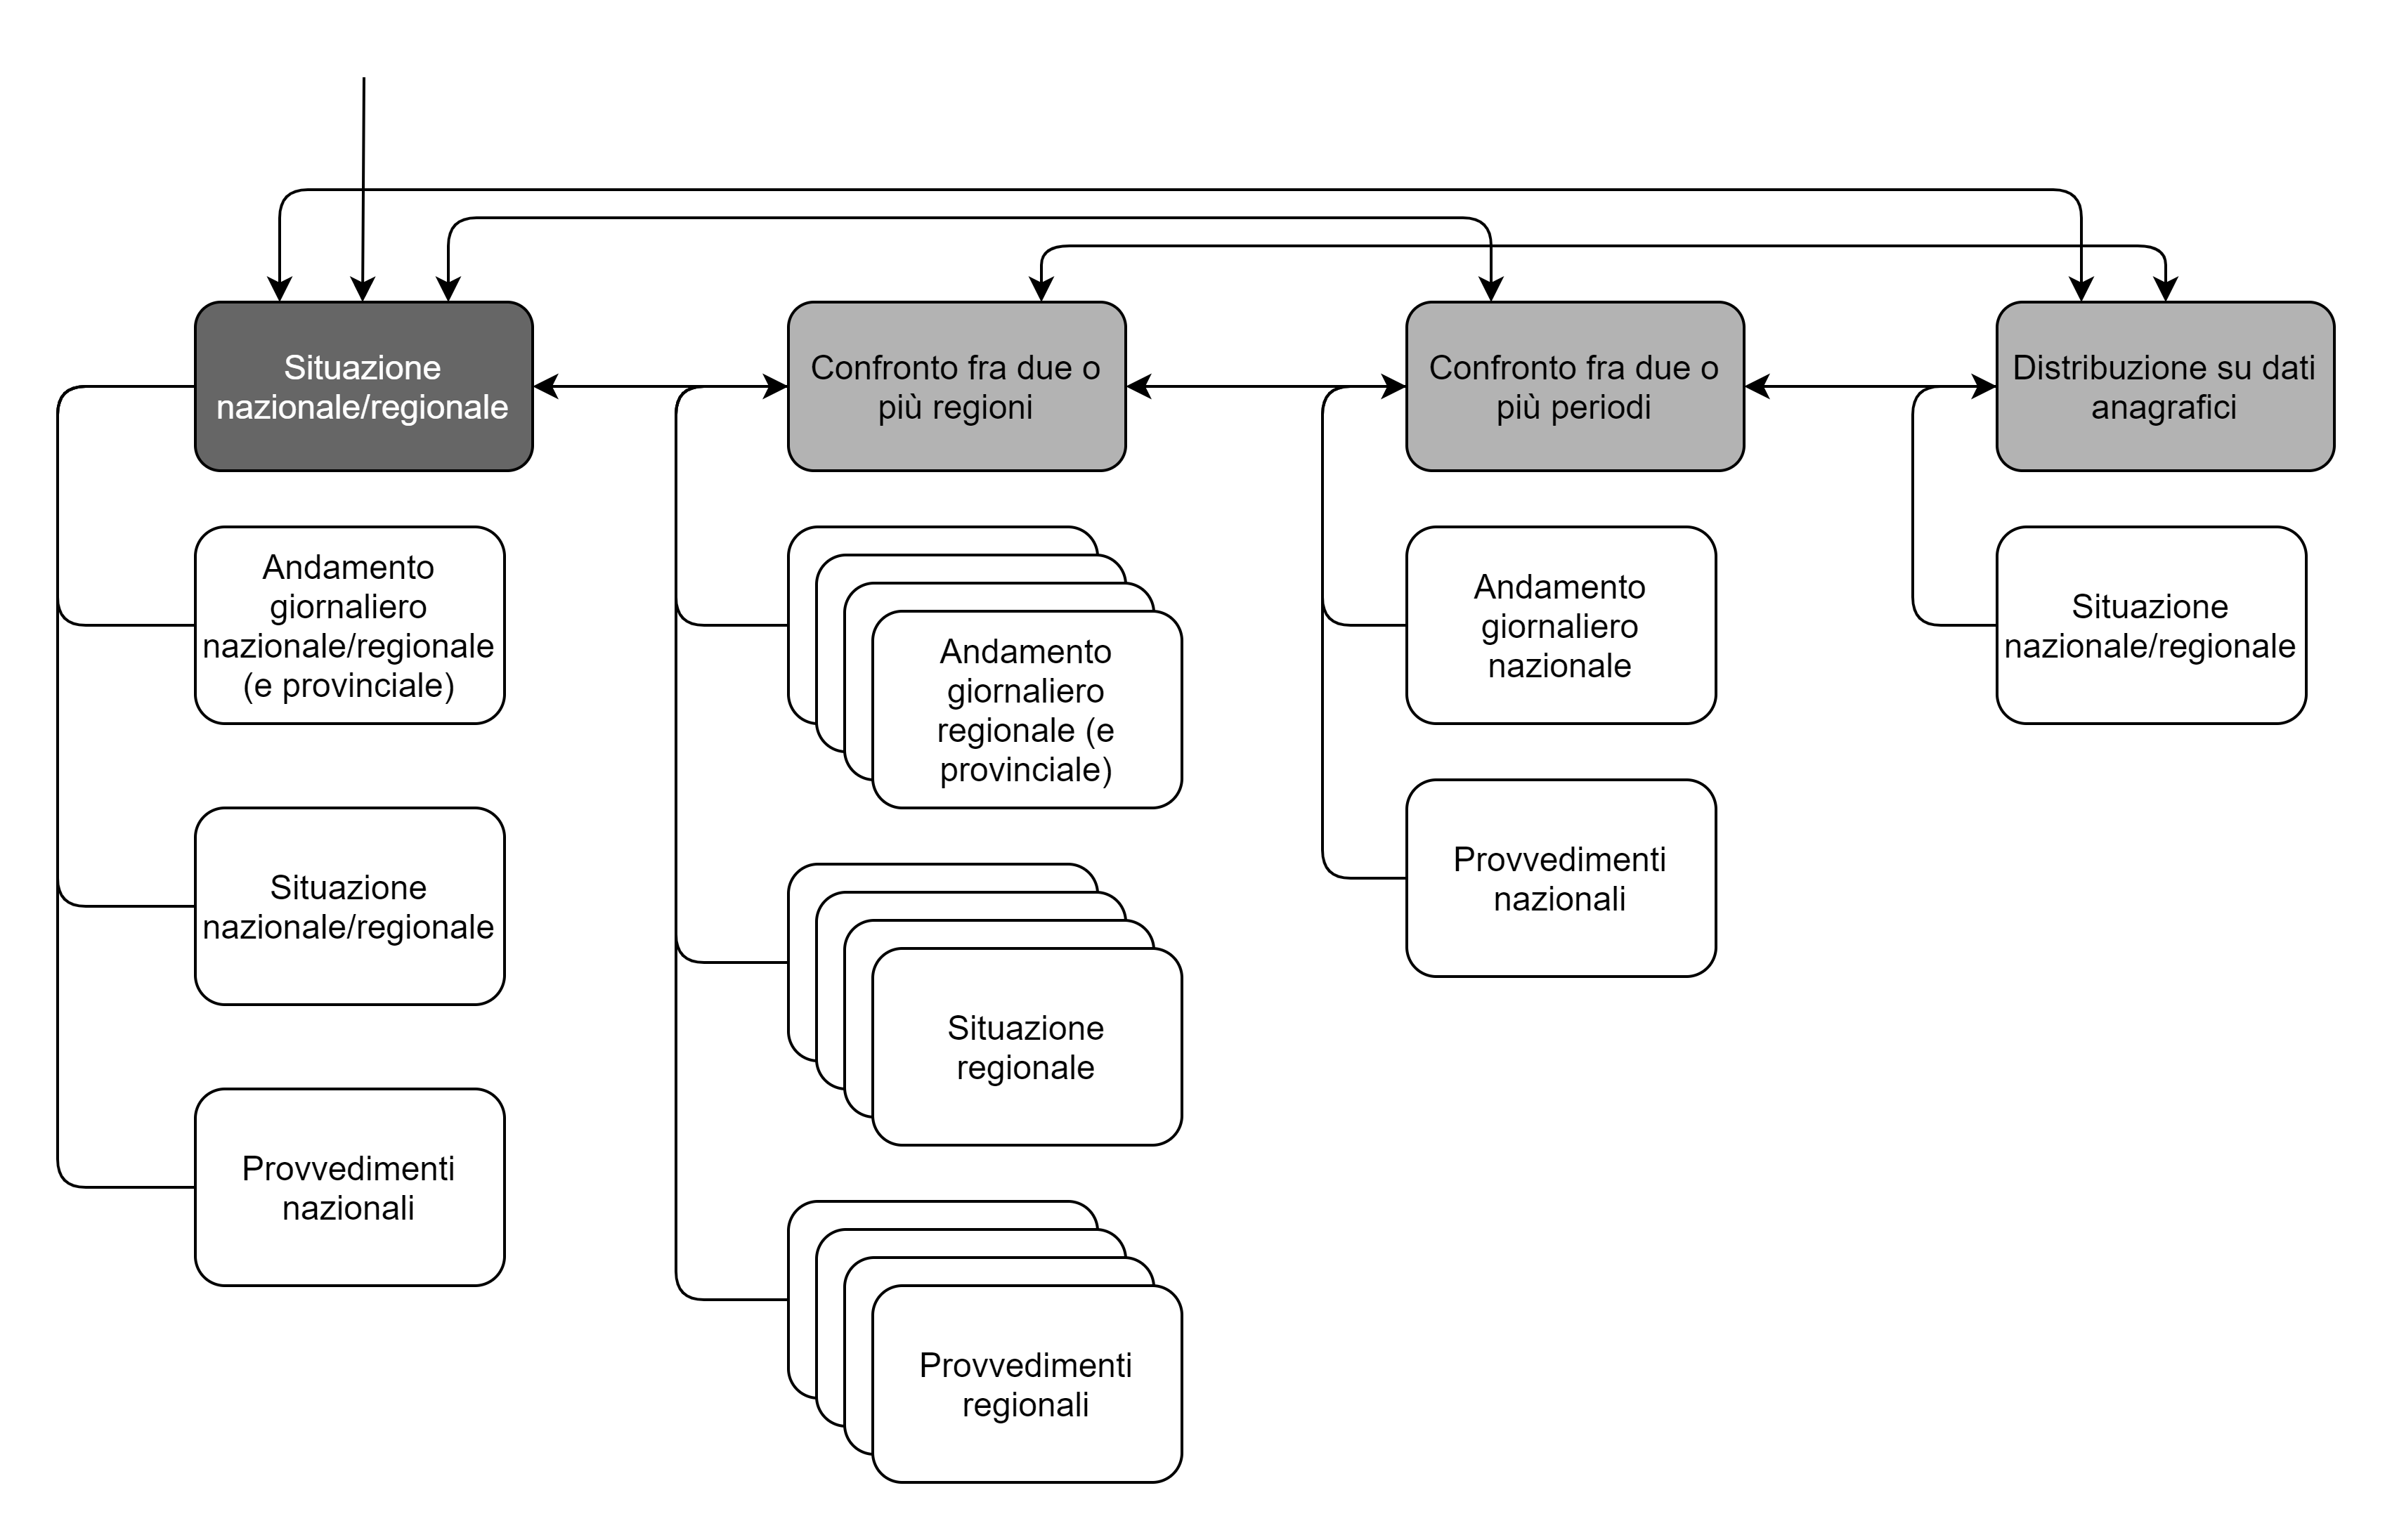
\includegraphics[width=5cm]{img/blueprint-cont-2}
					\end{column}
			\end{columns}
		\end{frame}

		\begin{frame}
			\begin{columns}[t]
					\begin{column}[T]{5cm}
						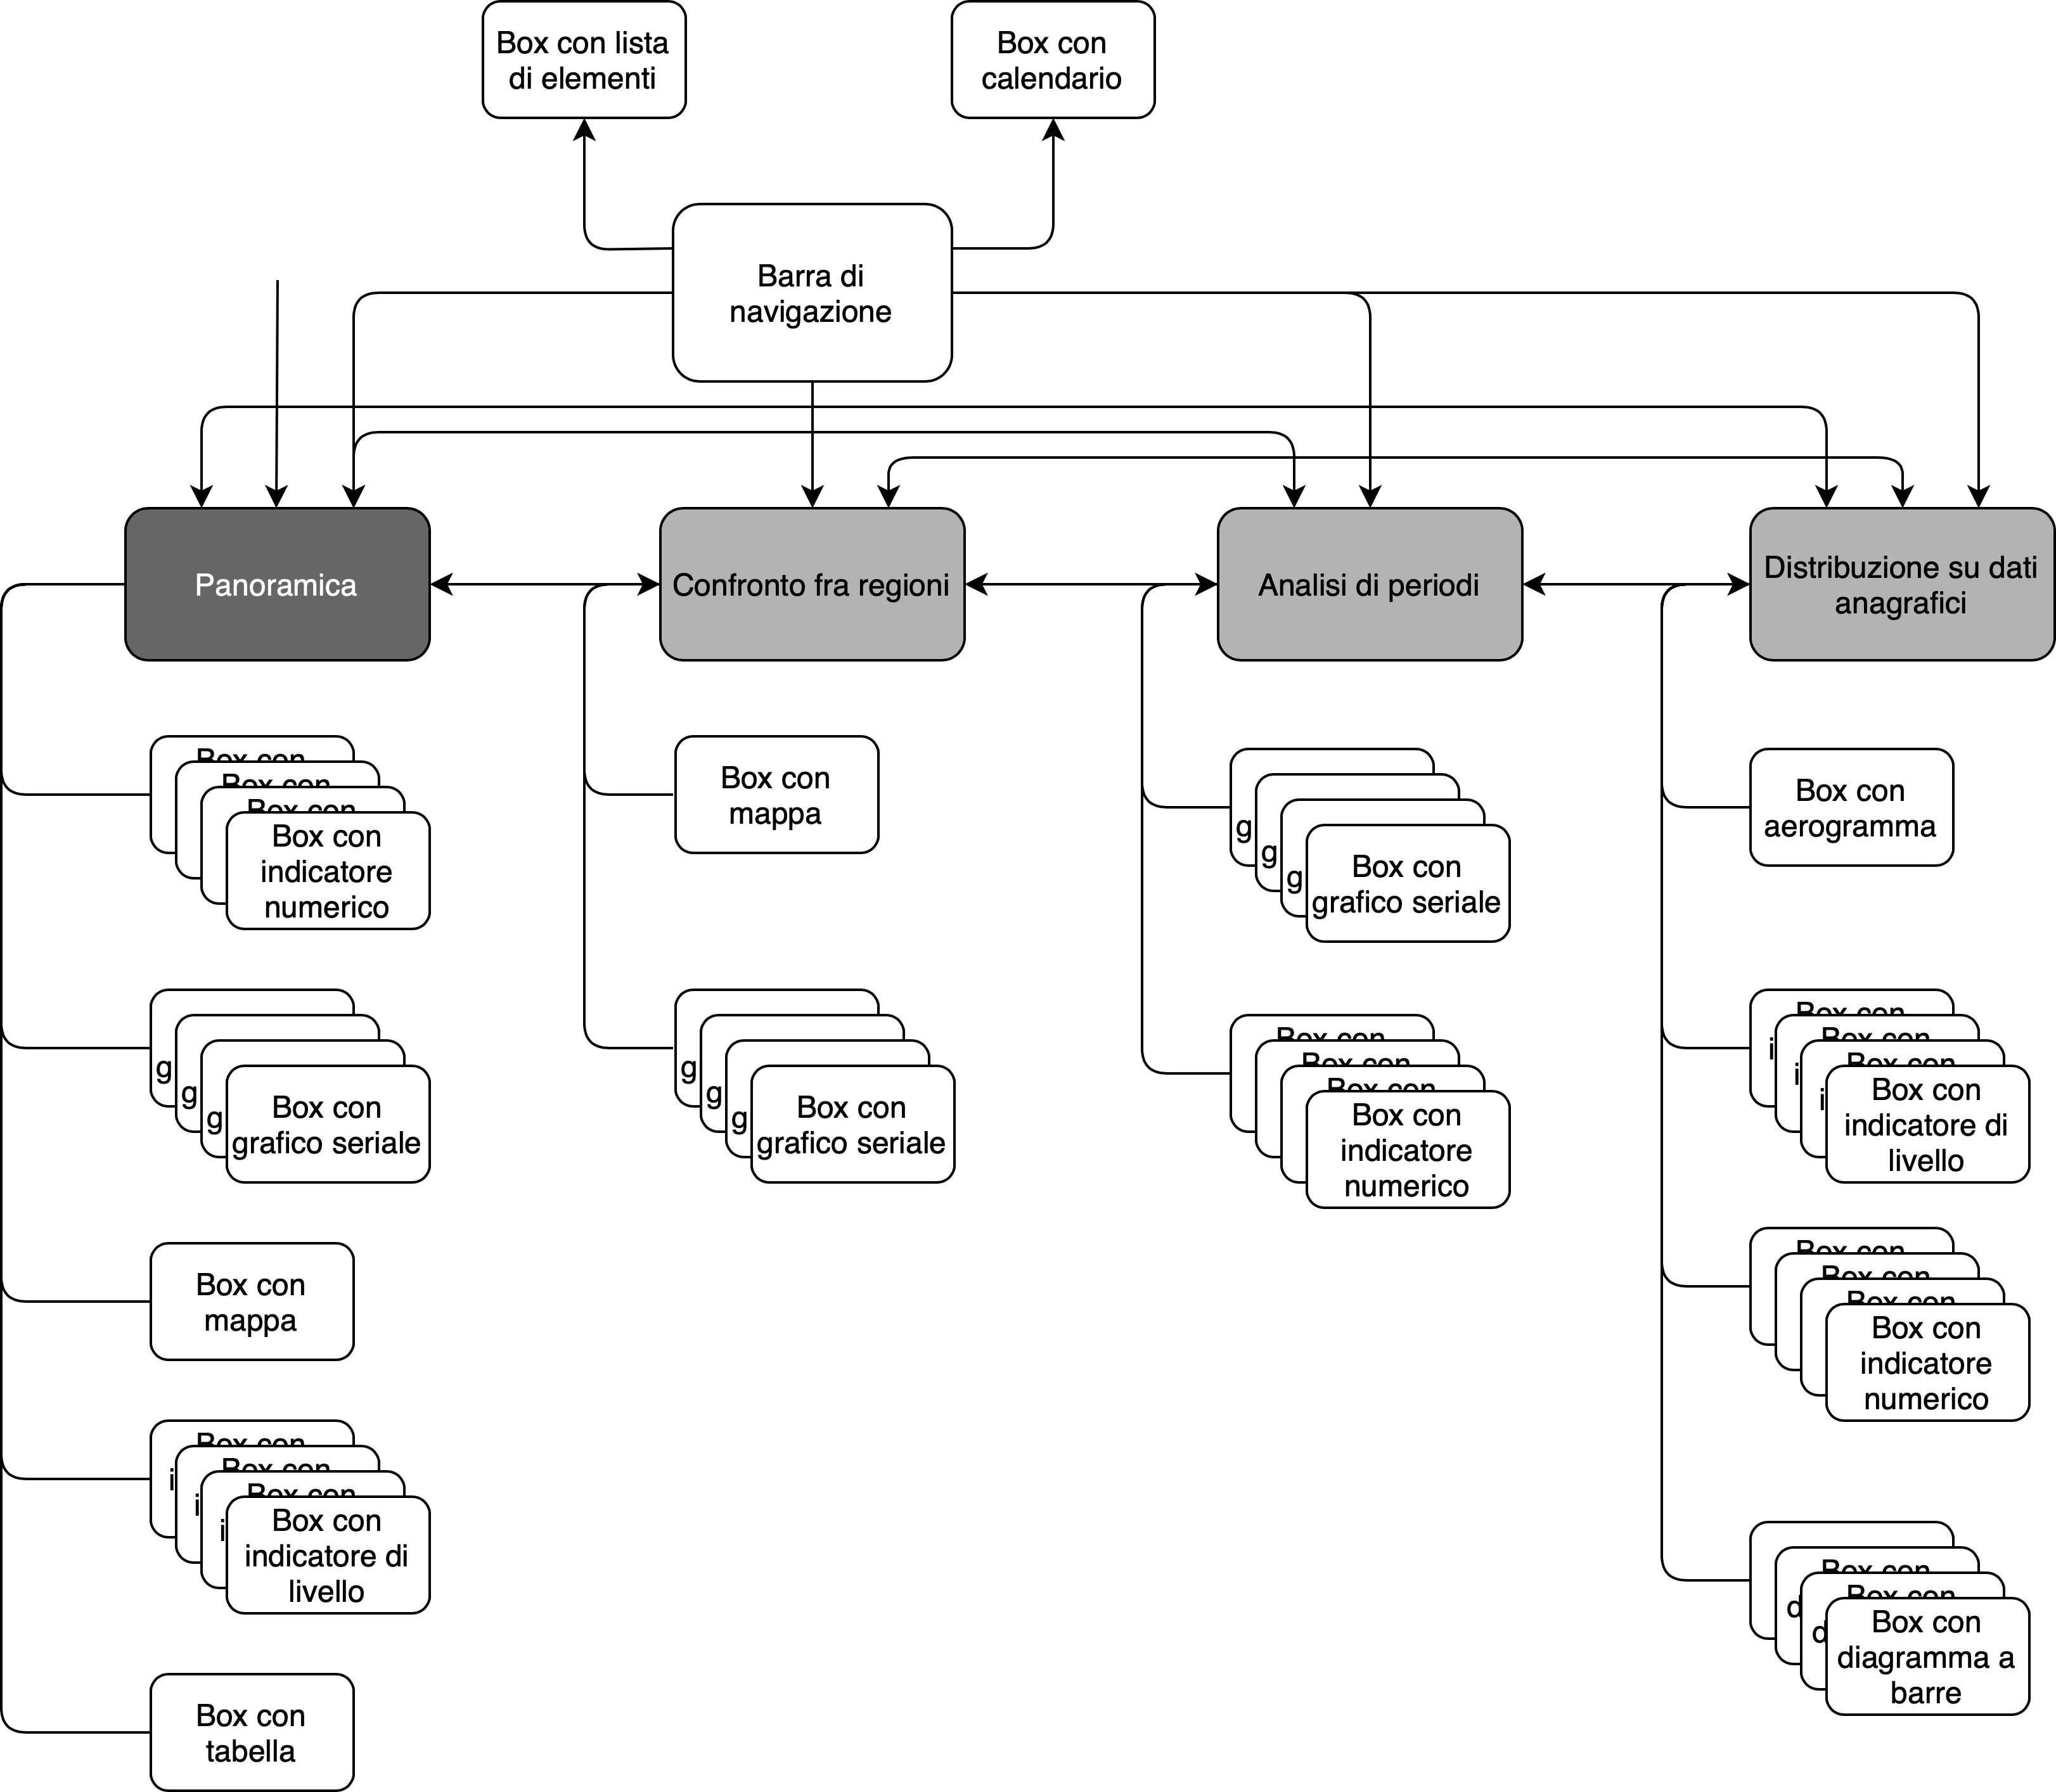
\includegraphics[width=5cm]{img/blueprint-prog-4}
					\end{column}
					\begin{column}[T]{5cm}
						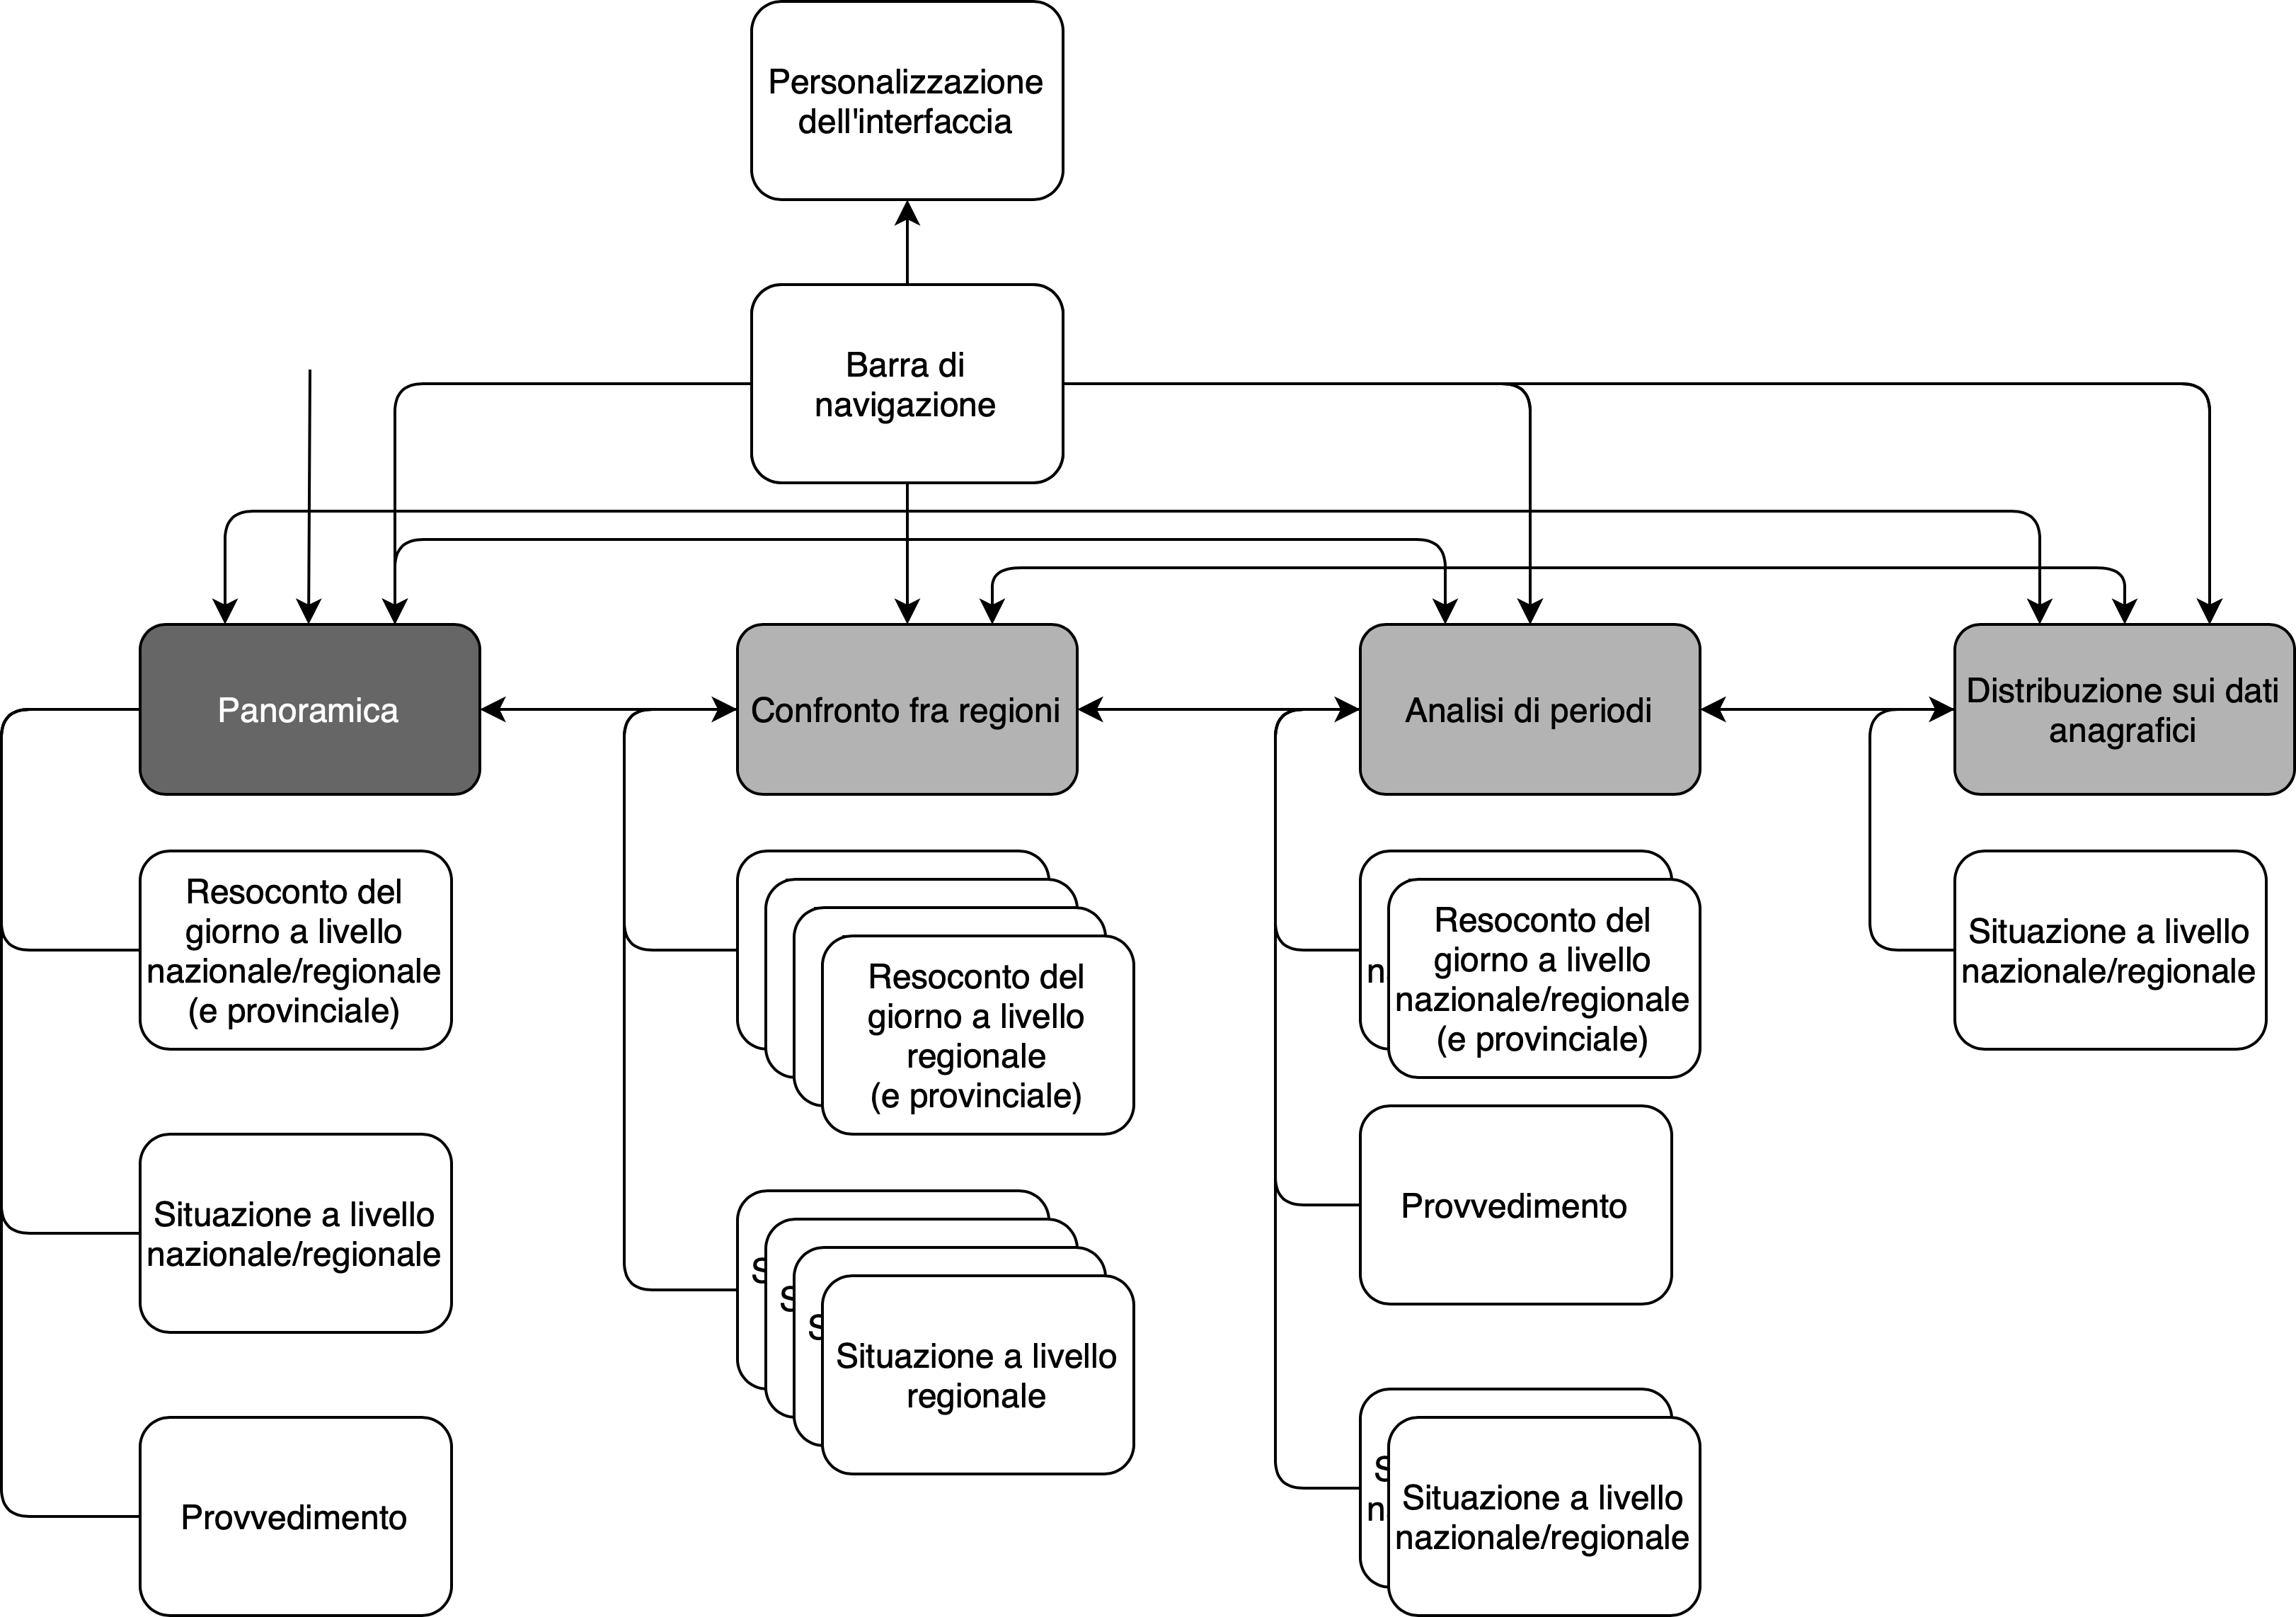
\includegraphics[width=5cm]{img/blueprint-cont-4}
					\end{column}
			\end{columns}
		\end{frame}


		\subsection{Wireframe}
		\begin{frame}
			\frametitle{Wireframe}
			Utilizzando Balsamiq abbiamo realizzato dei wireframe delle diverse pagine. 
		\end{frame}

		\begin{frame}
			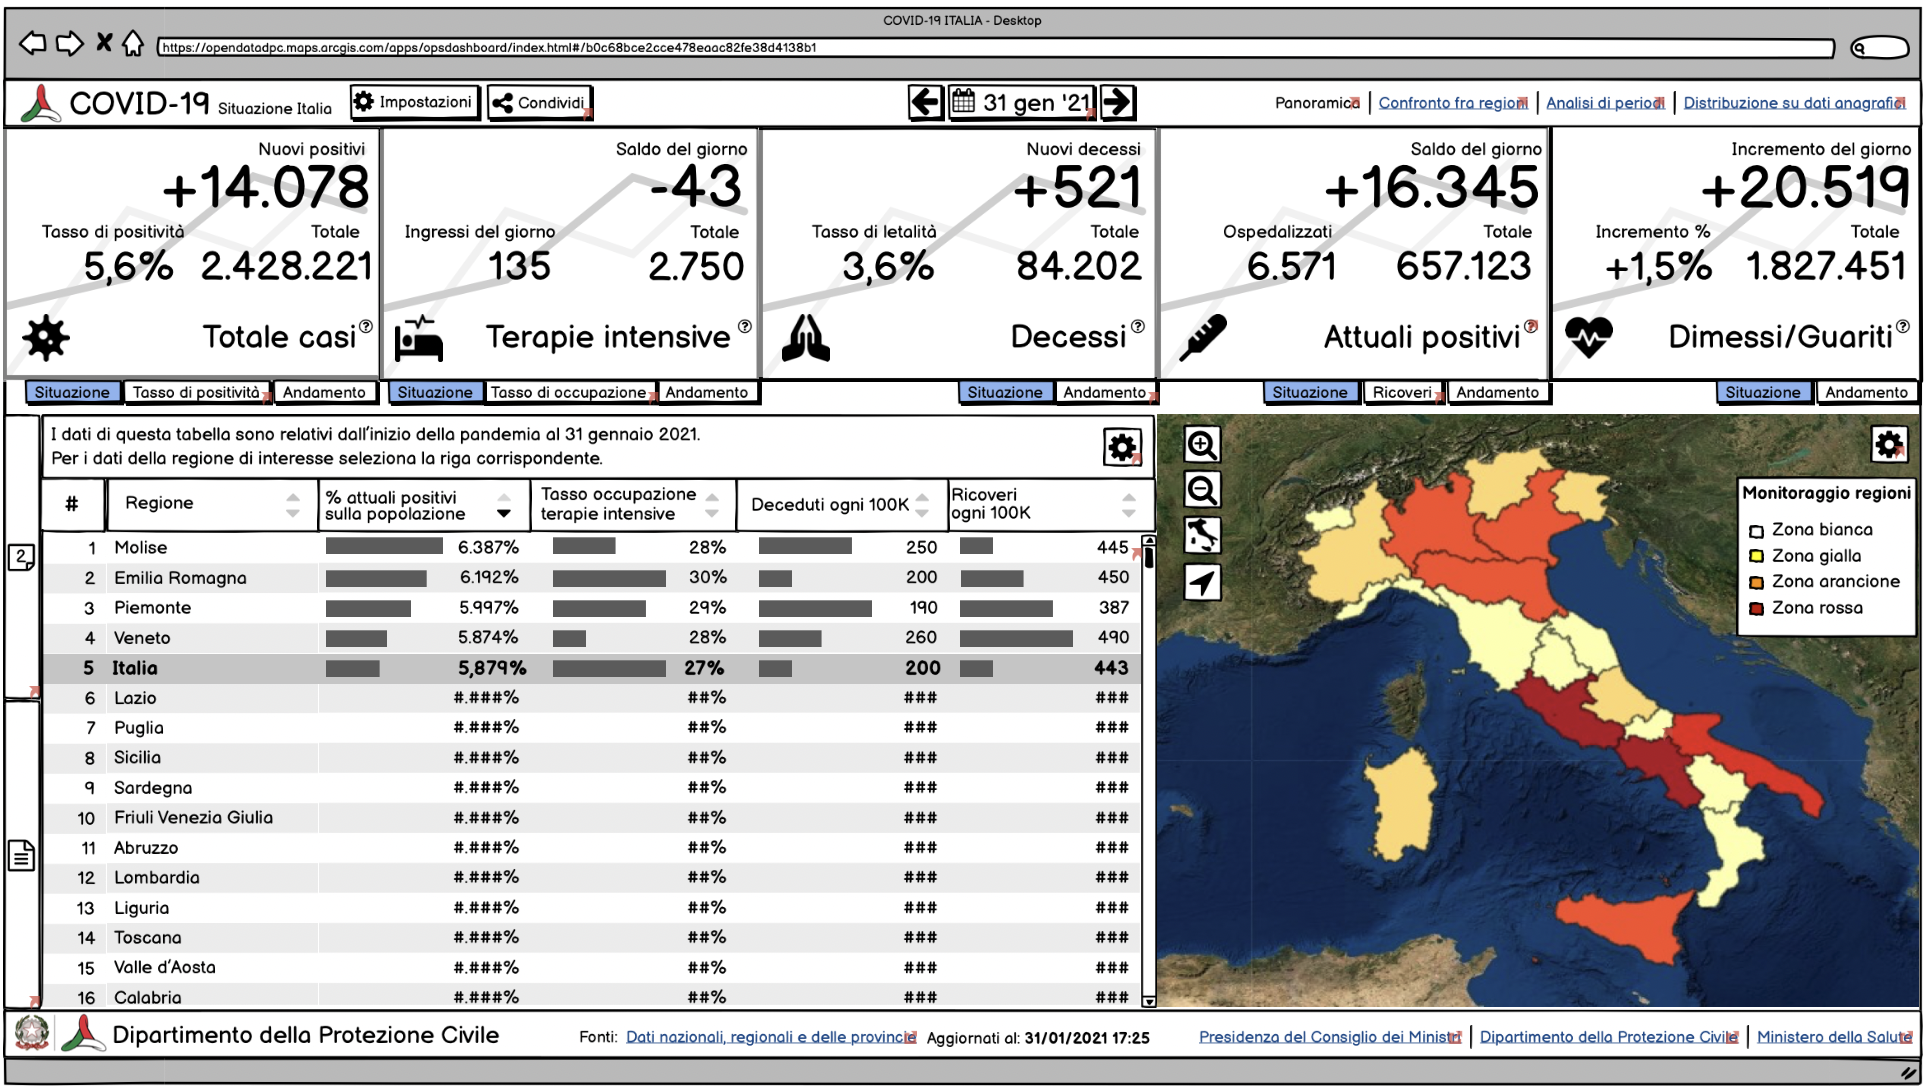
\includegraphics[width=10cm]{img/panoramica}
		\end{frame}

		\begin{frame}
			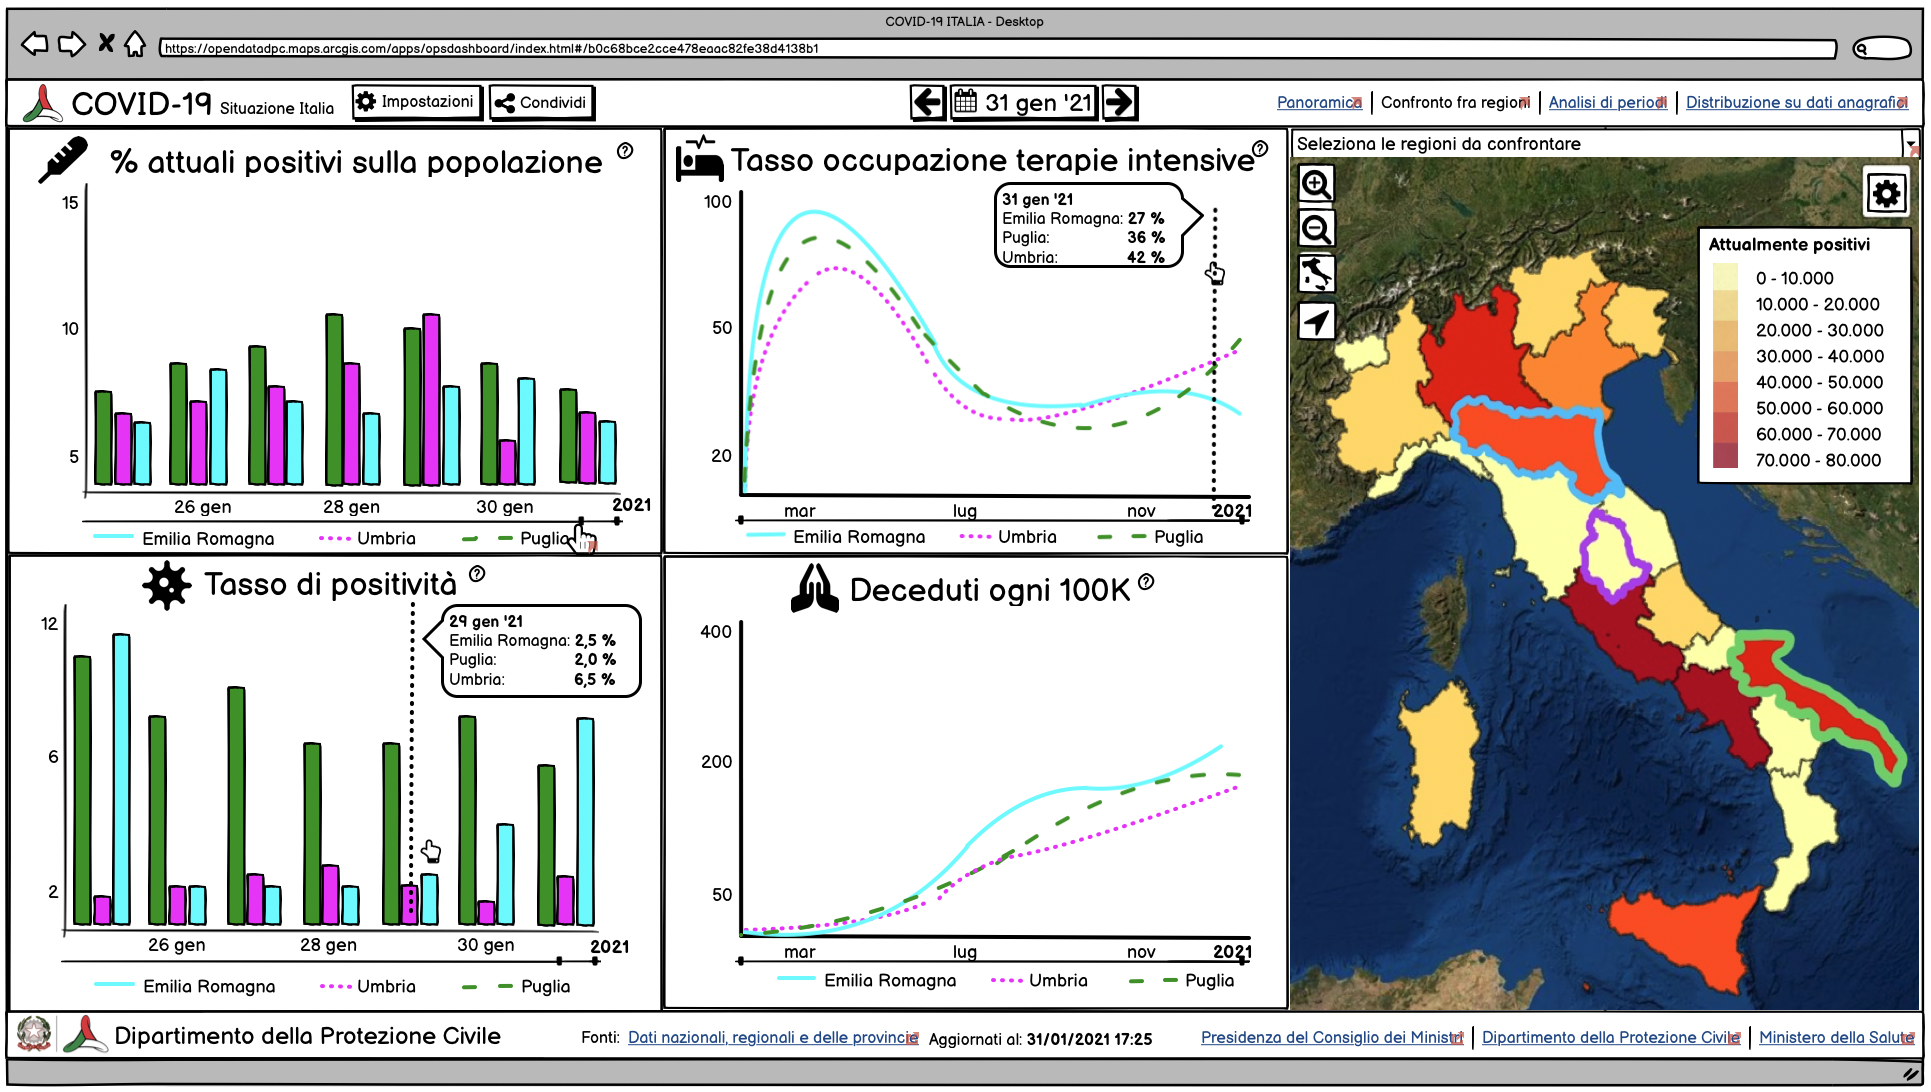
\includegraphics[width=10cm]{img/confronto-regioni}
		\end{frame}

		\begin{frame}
			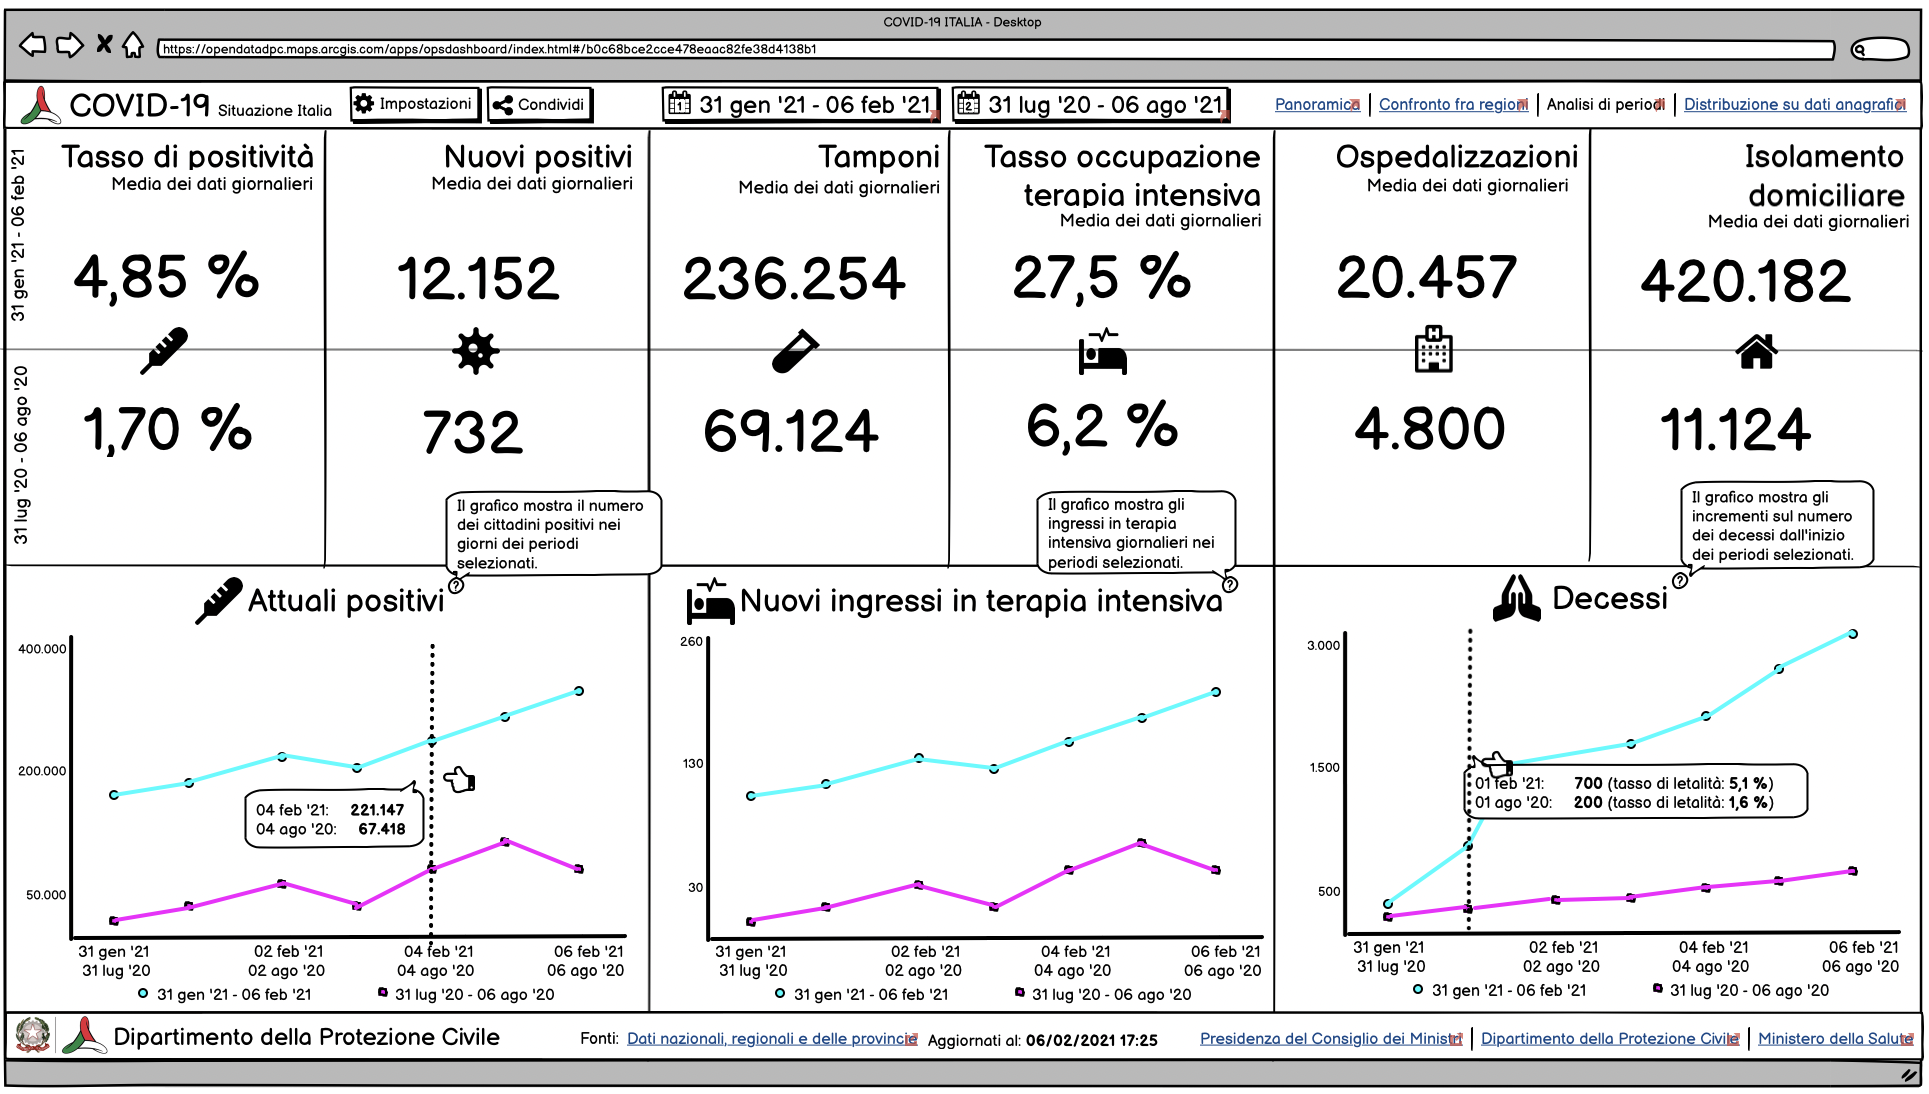
\includegraphics[width=10cm]{img/new-analisi-periodi}
		\end{frame}


		\begin{frame}
			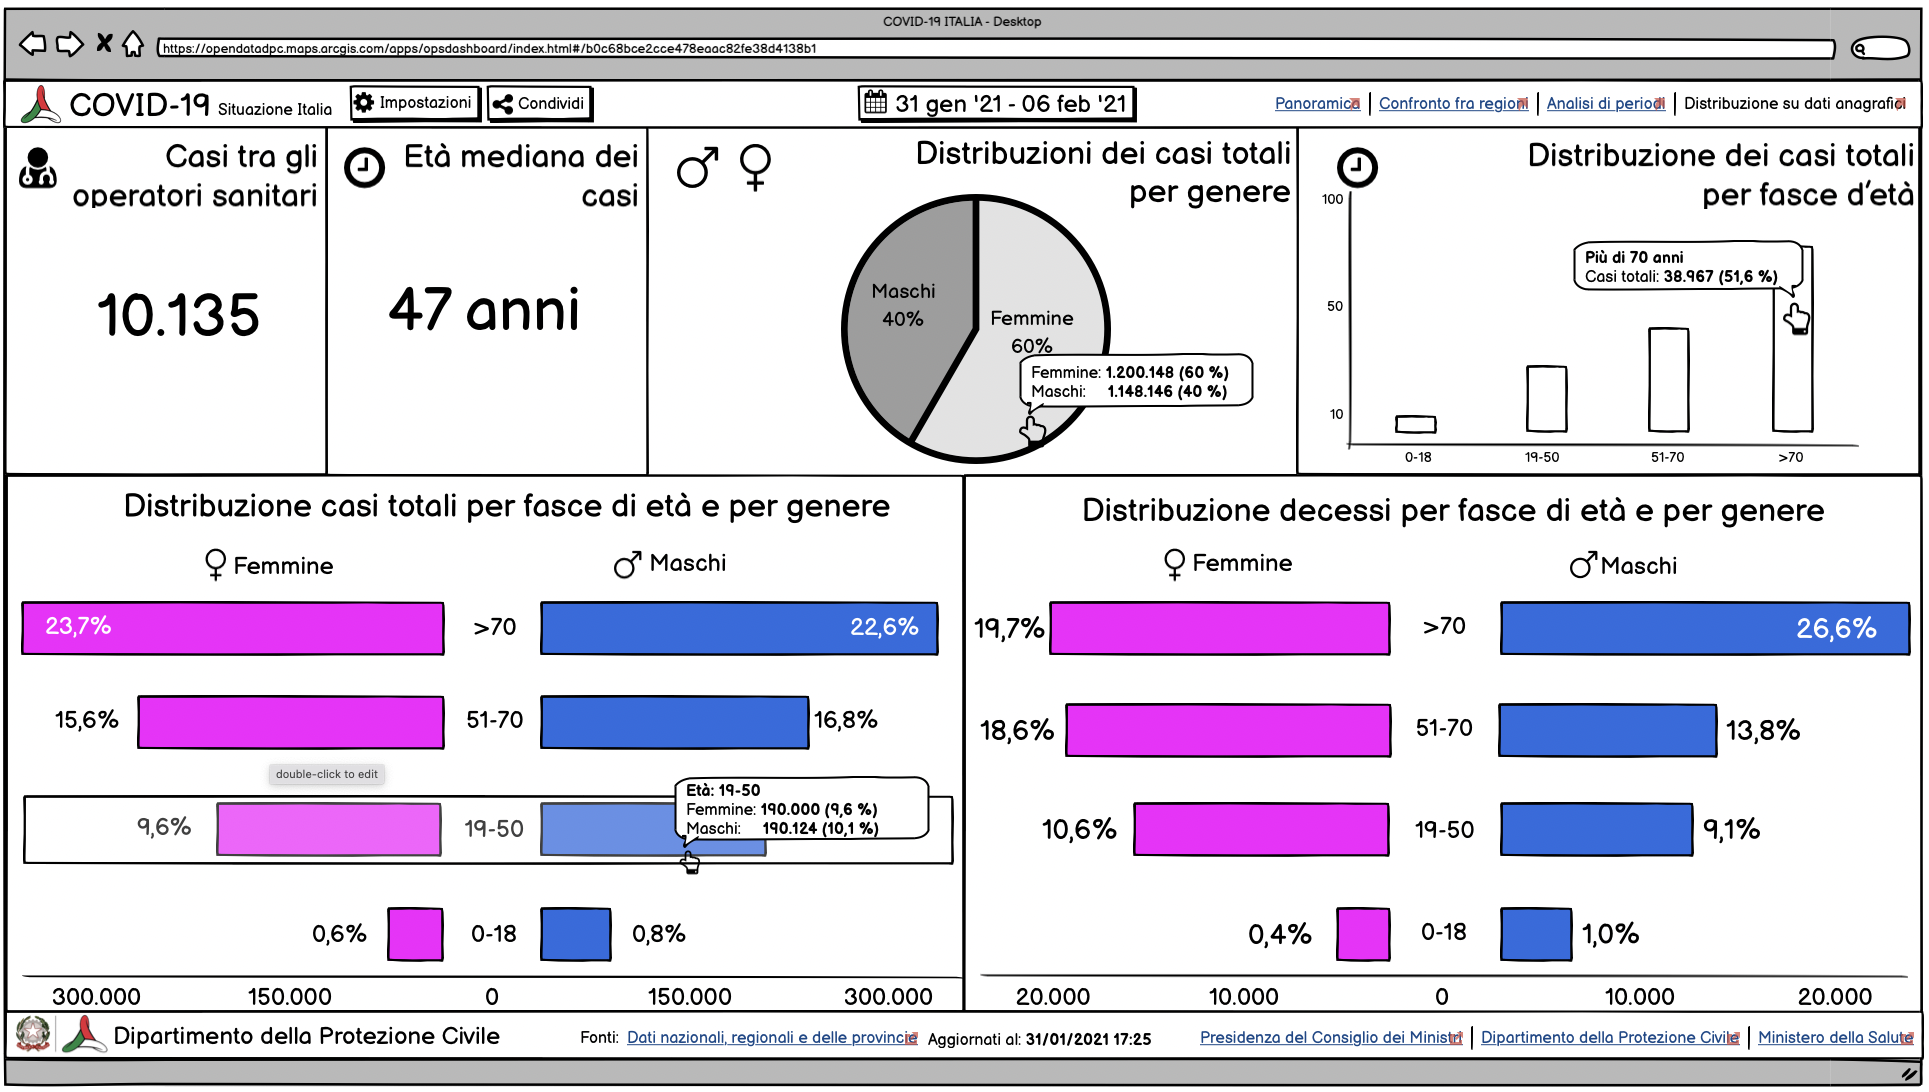
\includegraphics[width=10cm]{img/distribuzione-dati-anagrafici}
		\end{frame}


	\section{Valutazione}
		\subsection{Ispezione}
		\begin{frame}
			\frametitle{Cognitive walkthrough}
			Abbiamo svolto i task con la tecnica del cognitive walkthrough individuando alcune problematiche presenti nei wireframe che abbiamo corretto in iterazioni successive:
			\begin{itemize}[<+->]
				\item Diminuito il carico cognitivo aggiungendo etichette o semplifico la comprensibilità di quanto scritto\\
				\item Aggiunti dati necessari al completamento di alcuni task\\
				\item Modificato funzionamento relativo alla personalizzazione e alla condivisione dell'interfaccia\\
			\end{itemize}
		\end{frame}

		\begin{frame}
			\frametitle{Informal Action Analysis}
			Abbiamo svolto i task misurando, in maniera informale, il timing delle singolo azioni atomiche. \newline \newline
			\begin{block}{Risultati informal action analysis}
			Le tempistiche da noi misurate sono state in linea con quanto avevamo immaginato.
		\end{block}
		\end{frame}

		\begin{frame}
			\frametitle{Heuristic Analysis}
			Abbiamo confrontato le linee guida individuate con la nostra ri-progettazione. \newline \newline
			\begin{block}{Risultati heuristic analysis}
				Abbiamo individuato nove violazione che abbiamo prontamente corretto in una successiva iterazione dei wireframe.
		\end{block}
		\end{frame}

		\subsection{Testing}
		\begin{frame}
			\frametitle{Testing con gli utenti}
			\begin{itemize}[<+->]
				\item Abbiamo adottato un approccio di tipo Guerrilla\\ 
				\item Abbiamo definito un protocollo\\
				\item Abbiamo definito quali task sottoporre agli utenti:
					\begin{itemize}[<+->]
						\item Calcolare il tasso di positività relativo al 17 novembre 2020\\
						\item Valutare l'occupazione delle strutture sanitarie al 17 novembre 2020\\
						\item Calcolare il tasso di letalità medio nel mese di aprile 2020\\
					\end{itemize}
				\item Abbiamo provato a eseguire i task individuati nel test pilota\\
				\item Abbiamo chiesto a tre giornalisti di eseguire un task adottando l'approccio \textbf{thinking aloud}\\
			\end{itemize}
		\end{frame}

		\begin{frame}
			\frametitle{Testing con gli utenti - risultati}
			Abbiamo individuato \textbf{6} problematiche che abbiamo prontamente corretto in una successiva iterazione dei wireframe:
			\begin{enumerate}[<+->]
				\item Non si riesce a individuare il valore relativo ai ricoverati con sintomi\\
				\item Il ``secondo valore'' presente in ogni box numerico della schermata ``Panoramica'' non viene individuato immediatamente\\
				\item Richiesta di poter distinguere tra tamponi molecolari e antigenici\\
				\item Alcune metriche scelte di default nella tabella in ``Panoramica'' si sono rivelate poco interessanti\\
				\item Il termine ``metriche'' si è rivelato poco chiaro\\
				\item Difficoltà nel comprendere la semantica dei pulsanti per l'import e l'export dell'organizzazione dell'interfaccia\\
			\end{enumerate}
		\end{frame}

	\section{Conclusioni}
		\begin{frame}
			\frametitle{Conclusioni}
			\begin{block}{Obiettivo raggiunto}
				Fornire il giusto contesto alle analisi dei giornalisti così da permetter loro di maturare comprensioni corrette e profonde delle metriche epidemiologiche
			\end{block}
			\begin{itemize}[<+->]
				\item Ricerca etnografica $\rightarrow$ esigenze e testimonianze dei giornalisti\\
				\item Analisi risorse esistenti $\rightarrow$ criticità e loro importanza\\
				\item Studio di fattibilità $\rightarrow$ contesto d'uso, task e persona\\
				\item Riprogettazione proposta $\rightarrow$ modello CAO=S, architettura delle informazioni, interazioni, blueprint e wireframe\\
				\item Inspection e testing $\rightarrow$ validazione di quanto ri-progettato mediante test interni al gruppo e interviste ai giornalisti\\
			\end{itemize}
		\end{frame}
\end{document}
